\documentclass[a4paper,10pt]{article}
\usepackage[a4paper, total={167mm, 245mm}]{geometry}

\usepackage[colorlinks,linkcolor=blue,bookmarks,bookmarksopen,pdfauthor=krom]{hyperref}

\usepackage{fontspec}
\setmainfont[BoldFont={fonts/epkgobld.ttf}]{epkaisho.ttf}

\graphicspath{{images/}}

\usepackage[normalem]{ulem}
\renewcommand{\ULthickness}{0.08em}

\usepackage[compact]{titlesec}
\titlespacing{\section}{0em}{*0}{*0}
\titlespacing{\subsection}{0em}{*0}{*0}
\titleformat{\section}{\normalfont\large}{\thesection}{0em}{}
\titleformat{\subsection}{\normalfont\large}{\thesection}{0em}{}

\setlength\parindent{1em}
\setlength\parskip{0em}
\renewcommand{\baselinestretch}{1.4}

\usepackage{fancyhdr}
\pagestyle{fancy}
\fancyhf{}
\renewcommand\headrulewidth{0pt}

\begin{document}

\fancyfoot[R]{\thepage}

\begin{flushright}
2016/3/26 版
\end{flushright}

\vspace{17.5em}

\LARGE
\textbf{\hskip 5em \,OpenToonz}\par
\textbf{\hskip 5em スタートアップマニュアル}\par
\textbf{\hskip 5em 仕上げ編}

\noindent\begin{picture}(0,0)
\put(0,24){
\includegraphics[width=5em]{OpenToonzLogo}}
\end{picture}

\newpage

\huge
\noindent \textbf{目次}\\[-0.5em]
\par
\large
\noindent \textbf{\uline{\hskip -6em \hskip 6em はじめに\hskip 14em}}\\
\small
■OpenToonz での主なファイルフォーマット \ \ p.3\\
■OpenToonz のインターフェイス \ \ \ \ \ \ \ \ \ \ \ \ p.3\\
□Room について \ \ \ \ \ \ \ \ \ \ \ \ \ \ \ \ \ \ \ \ \ \ \ \ \ \ \ p.3\\
□パネルカスタマイズ \ \ \ \ \ \ \ \ \ \ \ \ \ \ \ \ \ \ \ \ \ \ p.3\\
□ファイルブラウザのインターフェイス \ \ \ \ \ \ p.4\\[0.5em]
\par
\large
\noindent \textbf{\uline{\hskip -6em \hskip 6em スキャン\hskip 14em}}\\
\small
□GTS によるスキャン \ ※ 「GTS 取扱説明書」 を参照してください。\\[1.5em]
\par
\large
\noindent \textbf{\uline{\hskip -6em \hskip 6em トレース (Cleanup)\hskip 9em}}\\
\small
□tlv ファイルの作成 \ \ \ \ \ \ \ \ \ \ \ \ \ \ \ \ \ \ \ \ \ \ p.4\\
□アンチエイリアスをかけず、サイズの変更も行わずに tlv ファイルを作成する場合 \ \ p.8\\[2em]
\par
\large
\noindent \textbf{\uline{\hskip -6em \hskip 6em 仕上げ (InknPaint)\hskip 9em}}\\
\small
□Level を読み込む \ \ \ \ \ \ \ \ \ \ \ \ \ \ \ \ \ \ \ \ \ \ \ \ p.9 \ \ \ \ \ \ \ □操作の取り消し \ \ \ \ \ \ \ \ \ \ \ \ \ \ \ \ \ \ \ \ \ \ \ \ \ \ p.15\\
□Level を保存する \ \ \ \ \ \ \ \ \ \ \ \ \ \ \ \ \ \ \ \ \ \ \ \ p.9 \ \ \ \ \ \ \ □連番フレームの表示を送る \ \ \ \ \ \ \ \ \ \ \ \ \ \ \ \ p.16\\
□新規 Level ファイルを作成する \ \ \ \ \ \ \ \ \ \ \ p.9 \ \ \ \ \ \ \ □フレームの複製・削除 \ \ \ \ \ \ \ \ \ \ \ \ \ \ \ \ \ \ \ \ p.16\\
□パレットファイルを保存する \ \ \ \ \ \ \ \ \ \ \ \ \ \ p.9 \ \ \ \ \ \ \ □画像の表示切り替えに関するメニュー \ \ \ \ \ \ p.16\\
□Scene ファイルを読み込む \ \ \ \ \ \ \ \ \ \ \ \ \ \ \ \ p.10 \ \ \ \ \ \ □各種ウィンドウを表示する \ \ \ \ \ \ \ \ \ \ \ \ \ \ \ \ p.17\\
□Scene ファイルを保存する \ \ \ \ \ \ \ \ \ \ \ \ \ \ \ \ p.10 \ \ \ \ \ \ □パレットのスタイルを編集する \ \ \ \ \ \ \ \ \ \ \ \ p.17\\
□ファイルを閉じる・新規Sceneファイルを作成する p.10 \ □Studio Palette について \ \ \ \ \ \ \ \ \ \ \ \ \ \ \ \ \ p.18\\
□OpenToonz を終了する \ \ \ \ \ \ \ \ \ \ \ \ \ \ \ \ \ \ \ \ p.10 \ \ \ \ \ \ □Studio Palette 内でフォルダを作成・削除、\\
□セルの合成・クミ切り \ \ \ \ \ \ \ \ \ \ \ \ \ \ \ \ \ \ \ \ p.11 \ \ \ \ \ \ \ \ \ 新規パレットを作成する。 \ \ \ \ \ \ \ \ \ \ \ \ \ \ \ p.18\\
□色を絵から抽出する \ \ \ \ \ \ \ \ \ \ \ \ \ \ \ \ \ \ \ \ \ \ p.13 \ \ \ \ \ \ □画像を表示する \ \ \ \ \ \ \ \ \ \ \ \ \ \ \ \ \ \ \ \ \ \ \ \ \ \ p.20\\
□途切れた線を自動でつなぐ \ \ \ \ \ \ \ \ \ \ \ \ \ \ \ \ p.13 \ \ \ \ \ \ □タイムシートの編集を行う \ \ \ \ \ \ \ \ \ \ \ \ \ \ \ \ p.21\\
□線の修正をする \ \ \ \ \ \ \ \ \ \ \ \ \ \ \ \ \ \ \ \ \ \ \ \ \ \ p.13 \ \ \ \ \ \ □ペイントの際に使用する色見本を表示する \ \ p.21\\
□領域を塗りつぶす \ \ \ \ \ \ \ \ \ \ \ \ \ \ \ \ \ \ \ \ \ \ \ \ p.13 \ \ \ \ \ \ □ファイルをブラウズする \ \ \ \ \ \ \ \ \ \ \ \ \ \ \ \ \ \ p.22\\
□ブラシで描く \ \ \ \ \ \ \ \ \ \ \ \ \ \ \ \ \ \ \ \ \ \ \ \ \ \ \ \ p.13 \ \ \ \ \ \ □tlv のフレームを表示する \ \ \ \ \ \ \ \ \ \ \ \ \ \ \ \ p.22\\
□文字を入力する \ \ \ \ \ \ \ \ \ \ \ \ \ \ \ \ \ \ \ \ \ \ \ \ \ \ p.14 \ \ \ \ \ \ □連番画像を動画でプレビューする \ \ \ \ \ \ \ \ \ \ p.23\\
□線・塗り領域を消す \ \ \ \ \ \ \ \ \ \ \ \ \ \ \ \ \ \ \ \ \ \ p.14 \ \ \ \ \ \ □環境設定・キーボードショートカットを変更する p.23\\
□画像で選択した範囲をコピー/貼り付け、移動する p.14 \ □各種表示メニュー \ \ \ \ \ \ \ \ \ \ \ \ \ \ \ \ \ \ \ \ \ \ \ \ p.23\\
□ベクター画像を編集する \ \ \ \ \ \ \ \ \ \ \ \ \ \ \ \ \ \ p.15 \ \ \ \ \ \ □ウィンドウレイアウトを固定する \ \ \ \ \ \ \ \ \ \ p.23\\
□画像の表示に関わるツール \ \ \ \ \ \ \ \ \ \ \ \ \ \ \ \ p.15 \ \ \ \ \ \ □tlvファイルをtlv以外のファイル形式に変換する p.24\\[1em]
\par
\large
\noindent \textbf{\uline{\hskip -6em \hskip 6em 色指定 (PltEdit)\hskip 10em}}\\
\small
□色指定を行うためのシートファイルの作成 \ \ p.25\\
□必要なフレームのみを表示する \ \ \ \ \ \ \ \ \ \ \ \ p.25\\
□ダブラシ影などを透けた表示でプレビューする \ \ \ p.26

\fancyfoot[R]{\thepage
\begin{picture}(0,0)
\put(-523,-50){
\includegraphics[width=58em]{OpenToonzFooter}}
\end{picture}
}

\newpage

\phantomsection
\section*{\uline{■ OpenToonz での主なファイルフォーマット}}
\addcontentsline{toc}{section}{■ OpenToonz での主なファイルフォーマット}

\vspace{0.5em}
\normalsize
\ \ tnz: Xsheet ファイル\par
\ \ tlv: 画像ファイル\par
\ \ tpl: パレットファイル\par
\ \ hst: 履歴ファイル\par
\ \ cln: Cleanup の設定ファイル\par
\ \ tif: GTS でスキャンした画像ファイル\\
\\[-1em]
\small
※ tlvはToonz上では連番ファイルで表示されますが、Windowsブラウザ上では1ファイルとして扱われます。\\
Toonz では大きく分けて Scene と Level のファイルで構成します。\\
Scene = 1 カット単位\\
Level = 1 セル単位\\

\phantomsection
\section*{\uline{■ OpenToonz のインターフェイス}}
\addcontentsline{toc}{section}{■ OpenToonz のインターフェイス}

\noindent OpenToonz のインターフェイスは、1つの Room (ワークスペース)\\
に各機能のパネルを配置・表示して使用するソフトウェアです。\\[-3.8em]

\phantomsection
\subsection*{\hskip 23.5em □ Room について}
\addcontentsline{toc}{subsection}{□ Room について}

\footnotesize
\hskip 34em Room とは、各作業に特化したメニューやレイアウトを、\par
\hskip 34em タブ (画面右上に表示) で切り替えて作業を行う場所です。\\
\par
\hskip 34em [Cleanup]: tif 画像ファイルから tlv 画像ファイルを作成する\par
\hskip 34em [Pltedit]: BG(背景) 素材と tlv を重ねて色指定をする\par
\hskip 34em [InknPaint]: tlv に対して線修正や彩色をする\par
\hskip 34em [Xsheet]: シートを組んで絵を合成する\par
\hskip 34em [Batches]: 複数枚のフレームに対して自動的に連続処理を行う\par
\hskip 34em [Browser]: ファイルの表示・編集を行う

\large
\noindent\begin{picture}(0,0)
\put(-10,-190){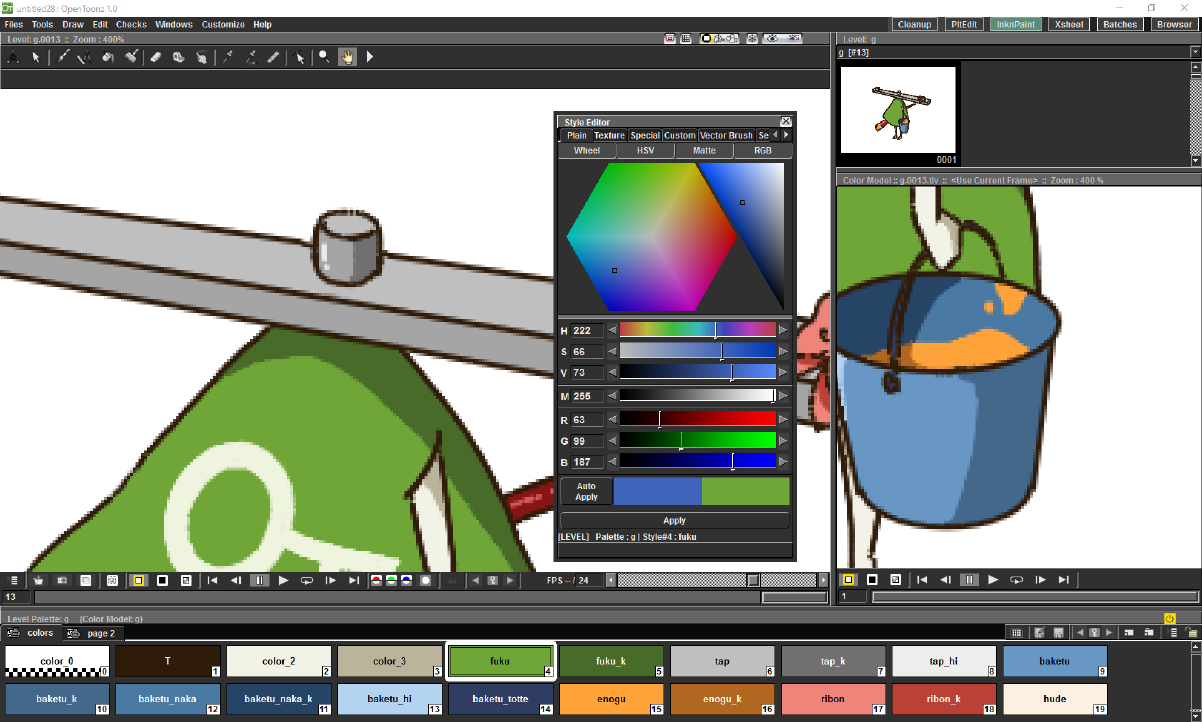
\includegraphics[width=28em]{OpenToonzInterfaceRoomPanels}}
\linethickness{0.1em}
\color{red}
\put(270,136){\line(1,0){102}}
\put(270,136){\line(-1,-5){26}}
\put(136,-222){\line(-1,0){142}}
\put(136,-222){\line(1,2){43}}
\end{picture}\\[15em]

\phantomsection
\subsection*{□パネルカスタマイズ}
\addcontentsline{toc}{subsection}{□ パネルカスタマイズ}

\footnotesize
\noindent ・個々のパネルは [Windows] メニューから選択して表示します。\\
・各パネルは、Room の中へドッキング表示することができます。各パネルのタイトルバーをドラッグして移動するとドッキングされ\\
る位置のガイドが表示され、マウスをはなすとドッキングレイアウトに切り替わります。\\
・ドッキングされたパネルをフローティングウィンドウに戻す場合は、[Customize > Lock Room Panes]のチェックを外し、タイトルバー\\
部分をドラッグして取り出します。\\
・誤った操作により固定ウィンドウを解除させたくない場合は [Customize > Lock Room Panes] のチェックを入れておきます。

\newpage

\phantomsection
\subsection*{\uline{□ファイルブラウザのインターフェイス}}
\addcontentsline{toc}{subsection}{□ ファイルブラウザのインターフェイス}

\small
\noindent ファイルブラウザとは、ファイルの保存・読み込みなどを行うパネルです。\\
左側にフォルダがツリー状に表示され、右側に選択したフォルダの中身が表示されます。

\large
\noindent\begin{picture}(0,0)
\put(108,-165){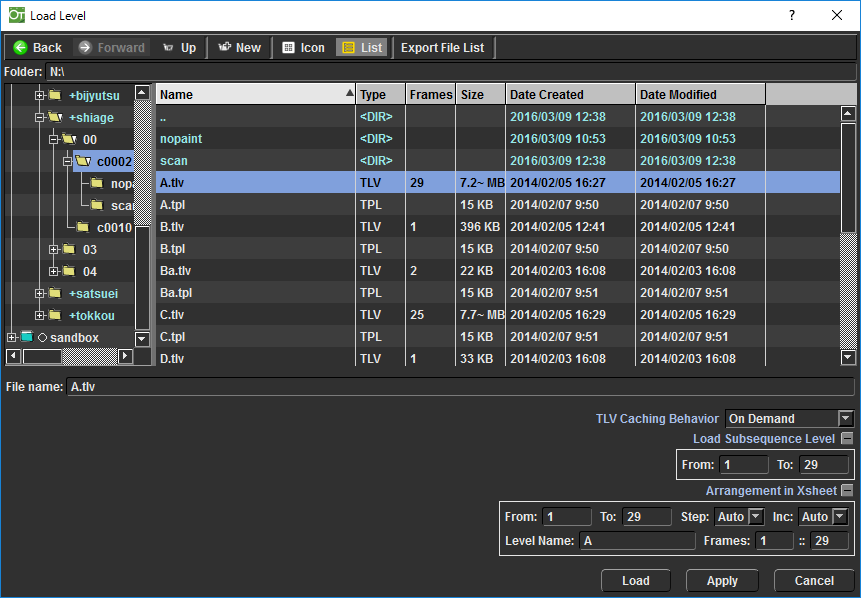
\includegraphics[width=21.2em]{OpenToonzInterfaceFileBrowserInterface}}
\end{picture}\\[12em]

\phantomsection
\section*{\uline{■ Cleanup (トレース)}}
\addcontentsline{toc}{section}{■ Cleanup (トレース)}

\small
\noindent Cleanup 工程では、GTS* でのスキャンで作成した tif 形式のファイルを使用し、ペイントファイル (Toonz ラスターレ\\
ベルファイル: tlv) を作成します。\\
※ GTS でのスキャンについては「GTS 取扱説明書」を参照してください。\\
Cleanup ルームに切り替えて作業を行います。\\
tlv の画像サイズ、切り出す画像の位置、線の濃さ、出力先の設定、書き出しなどを行います。\\

\phantomsection
\subsection*{\uline{□ tlv ファイルの作成}}
\addcontentsline{toc}{subsection}{□ tlv ファイルの作成}

\small
\noindent 1.GTS でスキャンした tif ファイルを Xsheet に読み込みます。

\large
\noindent\begin{picture}(0,0)
\put(116,-115){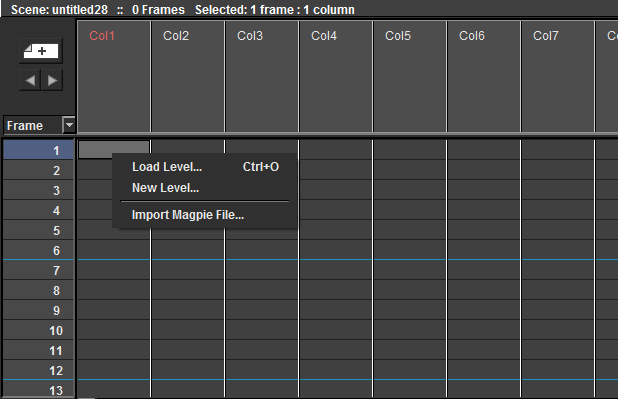
\includegraphics[width=20em,height=10.5em]{CleanupTLVFileCreationTIFImport}}
\end{picture}\\[8.2em]

\footnotesize
\noindent Xsheet 内で、tif を配置したいカラムを選択し、Files メニューもしくはカラムの右クリックメニューで Load Level を選択します。\\
※既に作成してある設定ファイル (cln) を読み込んで使用する場合は、tifファイルを選択し、Cleanup Settingsウィンドウ下の [Load]\\
から、設定ファイルを Load します。Load すると Cleanup Settings の値に反映されます。\\
\\
\small
2.プレビューしたい tif ファイルを選択します。\\
\footnotesize
レイアウト類→メインとなるセル→その他のセル の順に作業していきます。\\
プレビューしたい tif の上に他の絵が重なってしまう場合は [Camera Stand Visibility Toggle] で必要な絵のみ表示させます。\\
\\
\small
\uline{※手動でサイズの設定を行っていく場合は工程 3 へ。設定を読み込んで作業を行う場合は工程 5 へ。}\\
\\
3.tif 画像の角度が傾いている場合は正しい角度に直します。\\
\footnotesize
[Rotate]: 角度を選択し、Camera Test や Preview Cleanup を行うと、Rotate で選択した値が時計回りで反映されます。\\
\ [Flip]: 左右・上下に絵を反転します。

\newpage

\small
\noindent 4.Camera Test で Cleanup するサイズを設定する。\\
\footnotesize
\ [Processing/Camera Test] を選択します。Viewer の上に tif 画像と切り出す範囲を表す赤枠が表示されます。\\
□をドラッグで拡大縮小、赤枠範囲内でクリック \& ドラッグすると範囲の移動を行います。\\
Cleanup するキャンバスサイズを伸縮させても 現在の DPI を保持します。Resolution (ピクセルサイズ) はキャンバスサイズに合わ\\
せて変化します。\\
\ [Forced Squared Pixel]: ON のとき、1 ピクセルの縦横比を 1:1 にします。

\large
\noindent\begin{picture}(0,0)
\put(108,-144){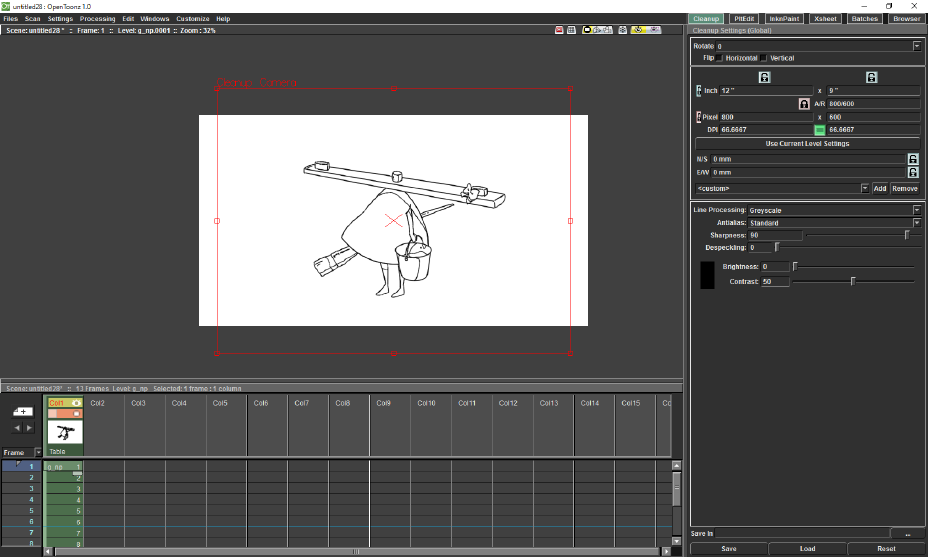
\includegraphics[width=21.7em]{CleanupTLVFileCreationCameraTest}}
\end{picture}\\[11em]

\small
\noindent 5.プレビューします。\\
\footnotesize
[Processing/Preview Cleanup] を選択します。\\
\\
\small
6.プレビュー画像に対して、線の処理、太さ、アンチエイリアスの適応具合を調節します。\\
\footnotesize
ライン処理が不要な場合は Line Processing オプションを None にします。ラインを黒として認識させたい場合は Greyscale を、色を認\\
識させたい場合は Color を選択します。

\large
\noindent\begin{picture}(0,0)
\put(145,-197){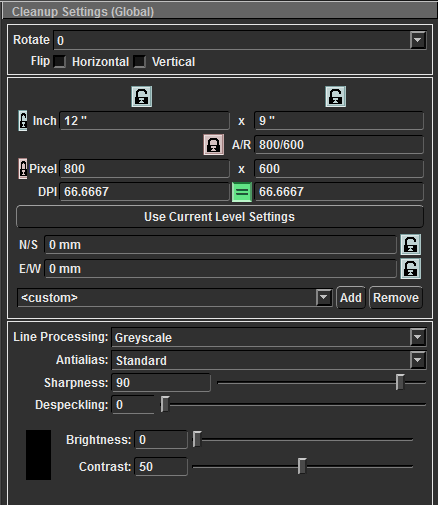
\includegraphics[width=15.3em]{CleanupTLVFileCreationCleanupSettings}}
\end{picture}\\[15em]

\footnotesize
\noindent アンチエイリアスの設定\\
\ [Standard]: スケールを変えることによるリサンプル処理でアンチエイリアスを付加します。\par
\ \ \ \ \ \ \ \ \ \ 出力結果の DPI を、元画像の 90%以下に縮めて処理を行うことが推奨されます。\\
\ [None]: アンチエイリアス処理を行いません。\\
\ [Morphological]: 画像のエッジを解析してスムージングします。画像サイズを縮める必要はありません。\\
\ [Brightness]: 線の太さが変化します。値が小さいほど、線は太くなります。\\
\ [Contrast]: アンチエイリアスの適用具合を調整します。大きい数値になるほどピクセルがはっきりとし、値が小さいほど、アンリエ\\
イリアスのかかったピクセルとなります。\\
アンチエイリアスの量は [Processing/Opacity Check] を有効にすることで確認できます。\\
※通常は Brightness と同じ値に設定します。Brightness の値以下に設定するとすべての線が半透明ピクセルになります。\\
※アンチエイリアスで None もしくは Morphological を設定した場合、Contrast パラメーターは機能しません。

\newpage

\noindent [Sharpness]: 線のシャープ度合いを定義します。値が大きいほどシャープで固いラインを生成します。低い値にすると、より滑らかな\\
ラインになります。\\
\ [Despeckling]: 画像から小さな斑点を削除します。値は除去される最大面積の大きさをピクセル単位で表示したものです。\\
Opacity Check を有効にすると除去される斑点の確認ができます。\\
\ [MLAA Intensity]: アンチエイリアスのMorphologicalにおけるぼかし強度を設定します。数値が大きいほどぼやけたラインになります。\\
(Morphological 選択時のみ利用可能)\\
\\
\small
カラー線画の場合、パラメーターを調整し、画像の中でどの色がどのように分かれているかを検出できるようにします。\\
\footnotesize
・Cleanup 処理後に自動的に線に割り当てられる色を設定します。\\
認識に使われる色と、認識後に割り当てられる色は Style Editor の下にあるボックスからどちらを編集するか選択し、それぞれ色を変\\
更することができます。①が認識に使われる色で、②が割り当てられる色のボックスです。RGB Picker ツールで作業エリアの画像から\\
色の値を拾うことも可能です。

\large
\noindent\begin{picture}(0,0)
\put(34,-233){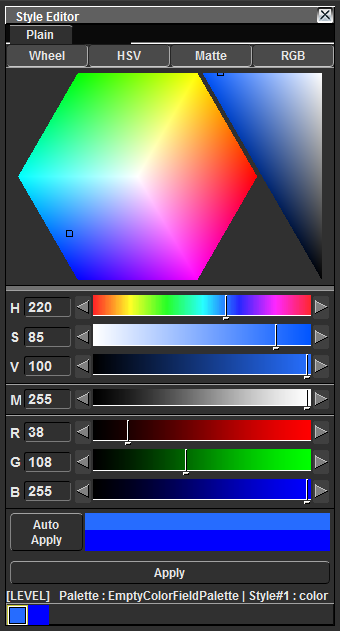
\includegraphics[width=11em]{CleanupTLVFileCreationStyleEditor}}
\put(228,-323.5){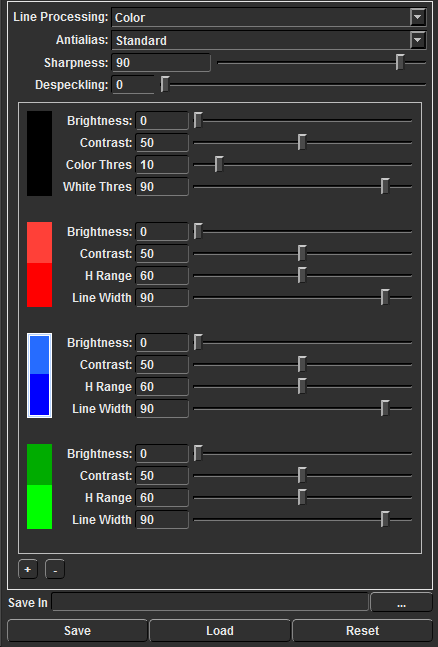
\includegraphics[width=18.9em]{CleanupTLVFileCreationLineProcessingColor}}
\put(206,-176.5){①}
\put(206,-196.5){②}
\put(34.5,-254){①}
\put(60,-254){②}
\linethickness{0.1em}
\color{red}
\put(213,-172){\line(1,0){29}}
\put(213,-192){\line(1,0){29}}
\put(34.5,-242){\line(0,1){13}}
\put(56,-242){\line(-1,1){13}}
\end{picture}\\[25.4em]

\footnotesize
\noindent ・黒色には異なるパラメーターを設定できます。黒は通常、線画の実線として定義されます。それ以外の色は通常、影やハイライトな\\
どの色トレス線として定義されます。\\
・カラーリストの追加・削除はカラーリスト下部分の [+][-] ボタンをクリックして行います。\\
・上記のパラメーターの他にカラーリストで設定できるパラメーターは下記になります。\\
\ [Color Threshold]: 黒と認識されるべきピクセル、およびカラーと認識されるべきピクセルについて設定します。値が大きいほど、カラー\\
とみなされるピクセルの量が多くなります。\\
\ [White Threshold]: 白とみなされるべきピクセルについて設定します。例えば紙の色を無視する場合などに使います。値が大きいほど、\\
白とみなされるピクセルの量が多くなります。\\
\ [H Range]: 色認識のための色相範囲を設定します。値が大きいほど、ピクセルの色は多くなります。\\
\ [Line Width]: 表示される色線の幅を設定します。値が大きいほど線が太くなります。\\
\par
\small
\noindent 7.線の処理の値が決まったら Cleanup Settings ウインドウ下にある [Save In] 項目に tlv の出力場所を指定します。\\

\newpage 

\noindent 8.[Save Settings] で [Cleanup Settings] を保存します。\\
\footnotesize
全ての設定が終わったら Cleanup Settings ウインドウ下の [Save] ボタンをクリックし、保存場所を指定して Cleanup の設定ファイ\\
ル (拡張子 cln) を保存します。\\
※ cln ファイルは必ず元となる tif ファイルと同じフォルダ階層に保存してください。\\
※すでに cln を作成してある tif を選択すると、その cln 値が自動で Load します。\\
Level 内の同じ名前、同じ場所に保存することで、アニメーションレベルで利用することもできます。この場合、設定は tlv を選んだ時\\
に自動的に表示され、その tlv が cleanup される際には常に使われます。\\
読み込まれた cln の設定はプロジェクトやシーンにおいて、デフォルトの設定となります。\\
\\
\small
9.次のセルを Cleanup する場合は手順 2~8 を繰り返します。\\
\\
10.すべてのセルの cln を保存したら、Xsheet データ全体を保存します。\\
\footnotesize
全ての cln の保存が済んだら [Files/Save Scene As] で Xsheet を保存します。\\
\\
\small
11.Cleanup を行います。\\
\footnotesize
\uline{【カット内の全ての tif を cleanup する場合】}\\
\ [Windows/Other Windows/Tasks] を選択し、Tasks ウィンドウを表示させます。\\
Tasksメニュー[Add Cleanup]ボタンをクリックするとダイアログが表示されるので、cleanupしたいtnzファイルを選択し、OKをクリッ\\
クします。\\
Tasks メニューに選択した tnz が登録されるので、登録されたタスクを選択します。\\
\ [Start] ボタンをクリックすると計算を開始します。\\
\\
計算の状態は [Status] で確認します。\\
\ [Suspended]: 一時停止\\
\ [Running]: 計算中\\
\ [Completed]: 計算が正常に終了\\
\\
\ [Status] が [Completed] になり計算が終わったら、Tasks メニューから Remove を選択し、登録した tnz を削除します。\\
\ [Files/New Scene] にし、再度 [Load Scene] でtnzファイルを読み込むと、Xsheet 上のtif表示 (水色) がtlv表示 (緑色) に更新されます。\\
\par
\hskip 27.5em \uline{【Xsheet で選択した tif のみ cleanup する場合】}\par
\hskip 28em Xsheet に配置した tif を選択し、[Processing/Cleanup] を選択すると、\par
\hskip 28em cleanup ダイアログが表示されます。\\
\par
\hskip 28em ①選択したフレーム数がプログレスバーとともに表示されます。\par
\hskip 28em ② Cleanup のビュー ON/OFF\par
\hskip 28em ③ [Cleanup]: 1 フレームだけ Cleanup します。\par
\hskip 28em \ \ \ [Skip]: 1 フレーム分だけ Cleanup をスキップします。(実行せず\par
\hskip 28em 次のフレームへ移動します。)\par
\hskip 28em \ \ [Cleanup All]: 全フレームを Cleanup します。\par
\hskip 28em \ \ [Cancel]: Cleanup をキャンセルします。

\large
\noindent\begin{picture}(0,0)
\put(16,-36){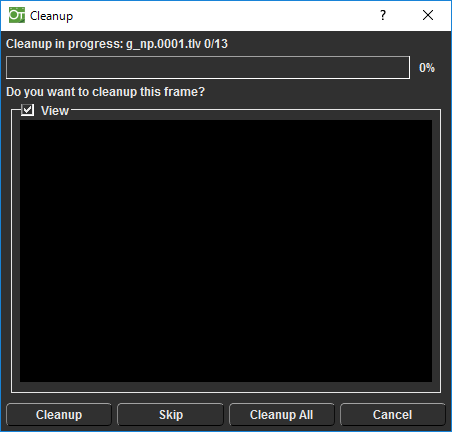
\includegraphics[width=17.3em]{CleanupTLVFileCreationCleanupFrame}}
\color{white}
\put(8,133){●}
\put(8,109){●}
\put(8,-33){●}
\color{red}
\put(8,133){①}
\put(8,109){②}
\put(8,-33){③}
\end{picture}\\[3em]

\small
\noindent 12.Cleanup の計算が終わったら、tlv が適正に作成されているか確認します。\\
\footnotesize
InknPaint Room にて [Files/Load Scene] を選択し、Cleanup した tnz を Load します。\\
Xsheet ウィンドウ上の tlv を選択し [ 右クリックメニュー /Info] を選択します。Image Size、Dpi の情報などを確認することができます。\\
Level Strip で動きを確認したいセルを選択し [Edit/Next Frame(Previous Frame)] でフレームの動きを確認します。

\newpage 

\phantomsection
\subsection*{\uline{□アンチエイリアスをかけず、サイズの変更も行わずに tlv ファイルを作成する場合}}
\addcontentsline{toc}{subsection}{□ アンチエイリアスをかけず、サイズの変更も行わずに tlv ファイルを作成する場合}

\small
\noindent ファイル変換機能により、tif や tga などの汎用画像連番ファイルから tlv を作成することもできます。\\
ファイルブラウザ上でコンバートしたいファイルを右クリックし、Convert...を選択します。

\large
\noindent\begin{picture}(0,0)
\put(3,-165){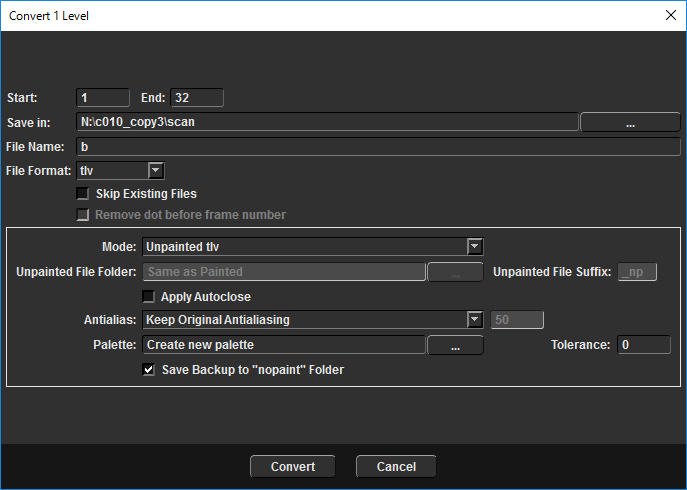
\includegraphics[width=19.2em]{WithoutAntialiasingConvert1Level}}
\color{white}
\put(19,-66.5){\small{●}}
\put(19,-76){\small{●}}
\put(28,-86){\small{●}}
\color{red}
\put(-6,-35){\footnotesize{①}}
\put(-6,-44){\footnotesize{②}}
\put(-6,-53){\footnotesize{③}}
\put(-6,-62){\footnotesize{④}}
\put(19,-66.5){\small{⑤}}
\put(19,-76){\small{⑥}}
\put(28,-86){\small{⑦}}
\end{picture}\\[12.6em]

\small
\noindent ①作成するフレーム範囲を入力します。\\
②作成する tlv の保存先を選択します。\\
③ファイル名を入力します。\\
④ファイル形式を選択します。tlv を作成する場合は tlv を選択します。\\
⑤チェックを入れると、保存先に既に tlv ファイルが存在している場合に、そのファイルには上書きせず新たにtlvを作\\
成します。\\
⑥チェックを入れると、変換前の tlv のファイル名のフレーム番号の前に付いている[.(ドット)]を削除することができ\\
ます。この機能は tlv のファイルから tga や他のファイル形式に変換する場合に使用します。\\
※変換後のファイル形式にtlvを選択していない場合のみ、機能が有効になります。詳細は「tlvファイルをtlv以外のファ\\
イル形式に変換する」 (p.23) をご覧ください。\\
⑦アンチエイリアスなしの\uline{線画の}連番画像ファイルから tlv に変換する場合は [\uline{Unpainted} tlv from non AA source]を\\
選択します。アンチエイリアスなしの、\uline{既に塗られた}連番画像ファイルからtlvに変換する場合は[\uline{Painted} tlv from non\\
AA source] を選択します。 既に塗られた連番画像ファイルを tlv に変換する場合は、塗りの境界に 1 ピクセルの線が自\\
動的に付加されて変換されます (見た目は変わりません)。

\newpage

\phantomsection
\section*{\uline{■ InknPaint}}
\addcontentsline{toc}{section}{■ InknPaint}

\noindent InknPaint ルームは、主に仕上げ工程において使用します。\\[-0.3em]

\phantomsection
\subsection*{\uline{□ Level を読み込む (Files/)}}
\addcontentsline{toc}{subsection}{□ Level を読み込む (Files/)}

\normalsize
\noindent Load Level…tlv を読み込むと、付随した tpl ファイルも読み込\\
まれます。\\[1.6em]
Load Folder…フレームの範囲を指定して Load する\\
機能です。\par
\footnotesize
\noindent From にフレーム始点、To にフレーム終点を入力します。\\
ペイント時、1つの tlv を複数人で作業するときは、こちらに各々が作業するフ\\
レームのみ入力します。\\
(※同じフレームを開いていると、Level を保存したときに、開いているすべて\\
のフレームが上書き保存されます。)\\
\par
\normalsize
\noindent Arrangement in Xsheet…Load する際に Xsheet への表示方法を\\
指定する場合に使用します。\par
\footnotesize
\noindent From にフレーム始点、To にフレーム終点を入力します。\\
Step は各フレームのコマ数を指定できます。\\
例) 1 と入力→ 1、2、3‥ 2 と入力→ 1、1、2、2、3、3‥\\
Inc は飛び石でフレームを省いて配置できます。\\
例) 2 と入力→ 1、3、5‥ 3 と入力→ 1、4、7‥\\
XsheetにはFrom、To で指定したフレーム数のみ表示されますが、tlvは全フレー\\
ム読み込まれます。

\large
\noindent\begin{picture}(0,0)
\put(295,29){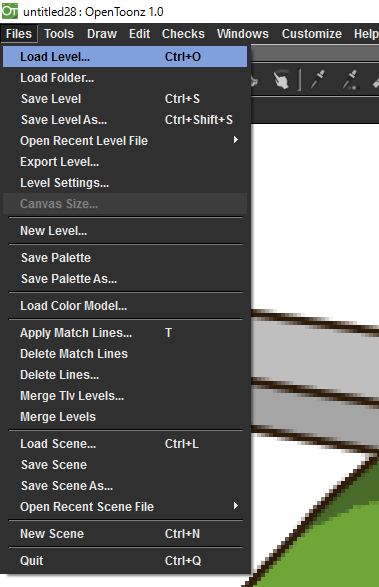
\includegraphics[width=14.8em]{InknPaintLevelFileLoading}}
\end{picture}\\[-2.7em]

\phantomsection
\subsection*{\uline{□ Level を保存する (Files/)}}
\addcontentsline{toc}{subsection}{□ Level を保存する (Files/)}

\normalsize
\noindent Save Level…現在選択している tlv を上書き保存します。\par
\footnotesize
\noindent 保存を実行したとき tpl( パレットファイル ) を保存していないと以下のアラートウィンドウが表示されます。\\
Overwrite Palette…tlv を保存し、さらに tpl も上書き保存します。\\
Don't Overwrite Palette…tlv は保存し、tpl は保存しません。\\[-0.7em]
\par
\normalsize
\noindent Save Level As…現在作業中の tlv ファイルを別名で保存します。\par
\footnotesize
\noindent tlv に付属する tpl も同時に保存します。(A.tlv を保存すると A.tpl も保存されます)\\[-1em]
\\
\normalsize
Open Recent Level File…過去に作業を行ったtlvが履歴として表示され、そのtlvを選択すると Load します。\\[-0.6em]
\\
Level Settings…現在選択中の tlv の情報が別ウィンドウで表示されます。\\[-0.5em]

\phantomsection
\subsection*{\uline{□新規 Level ファイルを作成する (Files/)}}
\addcontentsline{toc}{subsection}{□ 新規 Level ファイルを作成する (Files/)}

\noindent New Level…新規に tlv を作成することができます。\\[-0.7em]

\phantomsection
\subsection*{\uline{□パレットファイルを保存する (Files/)}}
\addcontentsline{toc}{subsection}{□ パレットファイルを保存する (Files/)}

\noindent Save Palette…現在選択中の tlv のパレットファイル (tpl) を上書き保存します。\par
\footnotesize
\noindent メニューを選択するとダイアログが表示されます。\\
Overwrite…tpl を上書き保存する\\
Don't Overwrite…tpl を保存しない\\
※保存先の Path が表示されます。\\[-1.2em]
\par
\normalsize
\noindent Save Palette As…現在選択中の tlv のパレットファイル (tpl) を別名保存します。

\newpage

\phantomsection
\subsection*{\uline{□ Scene ファイルを読み込む (Files/)}}
\addcontentsline{toc}{subsection}{□ Scene ファイルを読み込む (Files/)}

\noindent Load Scene…tnz を読み込みます。\\[-0.7em]

\phantomsection
\subsection*{\uline{□ Scene ファイルを保存する (Files/)}}
\addcontentsline{toc}{subsection}{□ Scene ファイルを読み込む (Files/)}

\noindent Save Scene…tnz を上書き保存します。\\
\\
Save Scene As…tnz を別名保存します。\\
\\
Open Recent Scene File…過去に作業を行ったtnzが履歴として表示され、そのtnzを選択するとLoadします。\\

\phantomsection
\subsection*{\uline{□ファイルを閉じる・新規 Scene ファイルを作成する (Files/)}}
\addcontentsline{toc}{subsection}{□ ファイルを閉じる・新規 Scene ファイルを作成する (Files/)}

\noindent New Scene…Scene(tnz) を新規に作成します。現在開いているファイルを閉じるときにも使用します。\\
\footnotesize
Scene データを保存していないと、変更点を上書き保存するか保存せずに閉じるかを選択するダイアログが表示されます。\\
Scene は保存せず現在開いているファイルを閉じるために行う場合は、[Discard] を選択します。\\
tlv に保存していない変更点がある場合は、確認のダイアログが表示されます。\\

\phantomsection
\subsection*{\uline{□ OpenToonz を終了する (Files/)}}
\addcontentsline{toc}{subsection}{□ OpenToonz を終了する (Files/)}

\normalsize
\noindent Quit…OpenToonz を終了します。\\
\footnotesize
データを保存していないと、変更点を上書き保存するか保存せずに閉じるかを選択するダイアログが表示されます。

\newpage

\phantomsection
\subsection*{\uline{□セルの合成・クミ切り}}
\addcontentsline{toc}{subsection}{□ セルの合成・クミ切り}

\small
\noindent OpenToonz では、Xsheet パネルを合成伝票のように扱うことで、直観的にセルの合成を行うことができます。\\
\ [Files/Apply Match Lines] を実行して 2 つの tlv の線を合成します。\par
\normalsize
\noindent \hskip -0.5em 【手順1】\\
\footnotesize
Xsheet に現在作業中のtlv(合成の子。Match Lineを適用したいtlv) の右隣に、Match Lineするtlv(合成の親。Match Lineのtlv) を\\
配置します。セルの合成伝票通りに Xsheet に並べることで各セル番号にまとめて線を貼り付けることが可能です。(※以下の画像は、\\
G8~13 に F1 の線を貼り付けたい場合のシートの並べ方です)\par
\normalsize
\noindent \hskip -0.5em 【手順2】\\[-0.5em]
\par
\footnotesize
\noindent \hskip 27.5em ㋐現在作業中の tlv(合成の子。Match Lineを適用したいtlv)\par
\noindent \hskip 27.5em ㋑Match Line する tlv(合成の親。Match Lineのtlv)\\[-5em]

\noindent \hskip 27.5em ○\par
\noindent \hskip 27.5em ○

\large
\noindent\begin{picture}(0,0)
\put(82,-135){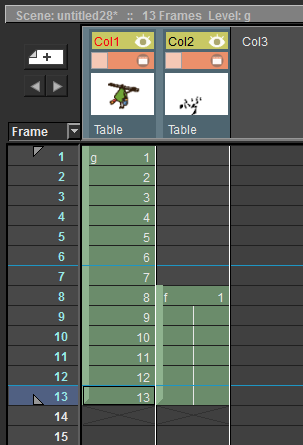
\includegraphics[width=10.7em]{InknPaintCellSynthesisCuttingXsheet}}
\color{white}
\put(128,32.5){\large{●}}
\put(159,32.5){\large{●}}
\color{red}
\put(128,32.5){\large{○}}
\put(159,32.5){\large{○}}
\put(128,32.5){\large{㋐}}
\put(159,32.5){\large{㋑}}
\end{picture}\\[9.5em]

\footnotesize
\noindent 両方のカラムを選択し、Apply Match Lines メニューを選択します。

\large
\noindent\begin{picture}(0,0)
\put(73,-215){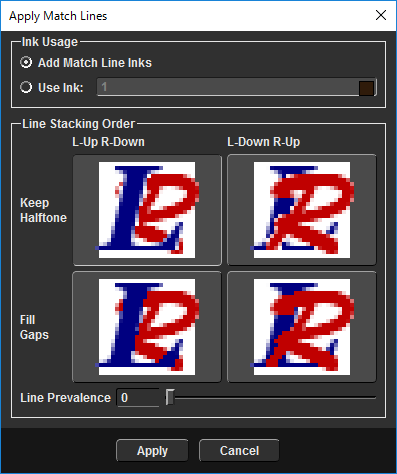
\includegraphics[width=15.2em]{InknPaintCellSynthesisCuttingApplyMatchLines}}
\put(307,-99){
\includegraphics[width=8.9em]{InknPaintCellSynthesisCuttingApplyMatchLinesLR}}
\color{white}
\put(70,-20){\normalsize{●}}
\put(70,-59){\normalsize{●}}
\put(344,-18.5){\large{●}}
\put(379,-24){\large{●}}
\color{red}
\put(70,-20){\normalsize{①}}
\put(70,-59){\normalsize{②}}
\put(344,-18.5){\large{○}}
\put(379,-24){\large{○}}
\put(344,-18.5){\large{㋐}}
\put(379,-24){\large{㋑}}
\end{picture}\\[15.5em]

\normalsize
\noindent \hskip -0.5em 【手順3】\\
\footnotesize
以下のウィンドウが表示されます。Match Lines をどの Ink で貼り付けるか、 どのくらい線を食い込ませるかを設定、実行します。\\
\small
① Ink Usage\par
\footnotesize
\noindent  [Add Match Line Inks]: Match Line する tlv で使用している線の色で貼り付けます。現在作業中のパレットに[match lines]というペー\\
ジが作成され、使用された色がコピーされます。\\
\ [Use Ink]: 現在作業中のスタイル番号を 1 つ指定し、その色で tlv を貼り付けます。\\
\\
※貼り付ける線を全て使用しない場合は、後で不要な線を削除できるように、実際に使用するスタイルではなく仮のスタイルを作成し\\
て貼り付けます。

\newpage

\footnotesize
\setlength{\arrayrulewidth}{0.1em}
\setlength{\tabcolsep}{0.5em}
\noindent \hskip 11em \begin{tabular}{|l|}
\hline
\small{L-Up R-Down・Keep Halftone}\\
\small{Line Prevalence [0]}\\
\scriptsize{・オリジナル 上・アンチエイリアスはそのまま}\\[-0.3em]
\scriptsize{・Match Lines下・アンチエイリアスはそのまま}\\[-0.3em]
\scriptsize{使用例)クミ線(BGクミ、セルクミ)、動画抜けの}\\[-0.3em]
\scriptsize{貼り付けなど}\\[1.5em]
\hline
\end{tabular}\\[-10.8em]

\noindent \hskip 41.5em \begin{tabular}{|l|}
\hline
\small{L-Down R-Up・Keep Halftone}\\
\small{Line Prevalence [100]}\\
\scriptsize{・オリジナル 下・アンチエイリアスはそのまま}\\[-0.3em]
\scriptsize{・Match Lines上・アンチエイリアスはそのまま}\\[-0.3em]
\scriptsize{使用例)合成子に影線・合成親に実線が描かれて}\\[-0.3em]
\scriptsize{いる場合の合成など}\\[1.5em]
\hline
\end{tabular}\\[0.5em]

\noindent \hskip 11em \begin{tabular}{|l|}
\hline
\small{L-Up R-Down・Fill Gaps}\\
\small{Line Prevalence [30]}\\
\scriptsize{・オリジナル 上・アンチエイリアスは Match}\\[-0.3em]
\scriptsize{Lines に侵食}\\[-0.3em]
\scriptsize{・Match Lines下・アンチエイリアスはそのまま}\\[-0.3em]
\scriptsize{使用例) 合成の貼り付けなど}\\[1.5em]
\hline
\end{tabular}\\[-10.8em]

\noindent \hskip 41.5em \begin{tabular}{|l|}
\hline
\small{L-Down R-Up・Fill Gaps}\\
\small{Line Prevalence [70]}\\
\scriptsize{・オリジナル 下・アンチエイリアスはそのまま}\\[-0.3em]
\scriptsize{・Match Lines上・アンチエイリアスはオリジナ}\\[-0.3em]
\scriptsize{ルに侵食}\\[-0.3em]
\scriptsize{使用例) 合成の貼り付けなど}\\[1.5em]
\hline
\end{tabular}

\large
\noindent\begin{picture}(0,0)
\put(5,94.6){
\includegraphics[width=6.6em]{InknPaintLineStackingOrderLRKeepHalftone}}
\put(250,94.6){
\includegraphics[width=6.6em]{InknPaintLineStackingOrderRLKeepHalftone}}
\put(5,4.5){
\includegraphics[width=6.6em]{InknPaintLineStackingOrderLRFillGaps}}
\put(250,4.5){
\includegraphics[width=6.6em]{InknPaintLineStackingOrderRLFillGaps}}
\end{picture}\\[-1em]

\small
\noindent ② Line Stacking Order\\
\footnotesize
Match Lines がどのくらいの食い込み具合で貼り付けるのかを設定します。\\
\ [Line Prevalence] がその設定です。0~100まで設定でき、0 は現在作業中の絵に全く影響を与えず Match Lines され、100は現在作\\
業中の線の上に Match Lines が完全に重なるように貼りつきます。\\
4つの選択窓は Line Prevalence でよく使う値をわかりやすいように表示したものです。\\
各ウィンドウをクリックすると値がそれぞれ、左上 [0]、右上 [100]、左下 [30]、右下 [70] になります。\\[0.7em]
\par
\normalsize
\noindent \hskip -0.5em 【手順4】\\
\footnotesize
クミ線の場合は、クミ線用にスタイルを新規作成します。必要な線の色を、作成したスタイルで塗り直します。\\
合成貼り付けの場合は、必要になる部分の線を実際に使用する線のスタイルの色に塗り直します。\\
※クミ線を塗り色に含みたくない場合は、クミ線のスタイルの Matte 値を 0 にします。\\[0.7em]
\par
\normalsize
\noindent \hskip -0.5em 【手順5】\\
\small
\ [Files/Delete Match Lines] メニューを実行し、現在選択している tlv の線を、スタイルを指定して消去します。\\
\footnotesize
メニューを選択すると以下のウィンドウが表示されます。\\
\ [Style Index]: 適用するスタイル番号を指定します。\\
\ [Apply to Frames]: 適用するフレーム番号を指定します。\\
※連続したフレームを指定したい場合は番号を [-(ハイフン)] でつなぎます。\\
例) 3 から 18 まで消去→ 3-18\\
※飛び石のフレームを指定したい場合は [,(コンマ)] で区切って入力します。\\
例) 1、3、6 フレームのみ消去→ 1,3,6

\newpage

\phantomsection
\subsection*{\uline{□色を絵から抽出する (Tools/)}}
\addcontentsline{toc}{subsection}{□ 色を絵から抽出する (Tools/)}

\large
\noindent\begin{picture}(0,0)
\put(0,0){
\includegraphics[width=1em]{ToolStylePicker}}
\end{picture}\\[-3.2em]

\normalsize
\noindent \ \ \ \ Style Picker Tool…tlv からクリックした部分の色の抽出・スタイル番号などの情報を知るための機能です。\par
\footnotesize
\noindent クリックする場所により、パレットのスタイルが連動します。Areas と Lines を個別に抽出することができます。ツールのショートカッ\\
トキーも個別に割り当てることができます。\\[-0.3em]

\large
\noindent\begin{picture}(0,0)
\put(0,0){
\includegraphics[width=1em]{ToolRGBPicker}}
\end{picture}\\[-3.2em]

\normalsize
\noindent \ \,\, RGB Picker Tool…tlv や tif など、Viewer に表示されている色 (RGB 値 ) を抽出する機能です。\par
\footnotesize
\noindent Normal 以外の Type を選択して使用すると、囲んだ範囲の平均 RGB 値を算出します。色は Style Editor に反映されます。\\
Passive Pick にチェックを入れておくと、カーソルの位置の RGB 値をリアルタイムでツールバーに表示します。\\[-0.3em]

\phantomsection
\subsection*{\uline{□途切れた線を自動でつなぐ (Tools/)}}
\addcontentsline{toc}{subsection}{□ 途切れた線を自動でつなぐ (Tools/)}

\large
\noindent\begin{picture}(0,0)
\put(0,0){
\includegraphics[width=1em]{ToolTape}}
\end{picture}\\[-3.2em]

\normalsize
\noindent \ \,\, Tape Tool…途切れている線画に対して、自動的に線をつなげる機能です。\par
\footnotesize
\noindent ある程度線が途切れている部分に対して実行すると、1 ピクセルの幅で線をつなぎます。\\
絵の種類によって Type を切り替え、数値を決めて使用します。\\
\ [Type - Normal]: クリックすると全画面に対して線つなぎを実行します。不要な部分もつながる可能性があります。\\
\ [Type - Rectangular、Freehand、Polyline]: 囲んだ範囲のみに線つなぎを実行します。\\
\ [Frame Range]: 複数のフレームに Tape Tool を実行します。\\
\ [Distance]: つなげられる最大のピクセル数を設定します。参考値) 50\\
\ [Angle]: つなげられる最大の角度を設定します。参考値) 90\\
\ [Style Index]: つなげる線の色を設定します。スタイル番号を入力するか、パレットのスタイルをクリックすることで変更できます。\\
\ [Opacity]: つなげる線の濃度を設定します。アンチエイリアスの無い二値でのペイント時には 255 にします。アンチエイリアスのあ\\
る絵での参考値は 25 です。\\[-0.3em]

\phantomsection
\subsection*{\uline{□線の修正をする (Tools/)}}
\addcontentsline{toc}{subsection}{□ 線の修正をする (Tools/)}

\large
\noindent\begin{picture}(0,0)
\put(0,0){
\includegraphics[width=1em]{ToolFinger}}
\end{picture}\\[-3.2em]

\normalsize
\noindent \ \ \ \ Finger Tool…線画に対して使用します。線画の上をなぞると、三方を囲まれた穴を埋めることができる\\
機能です。\par
\footnotesize
\noindent 基本は選んでいる色を使用しますが、線の上でクリックすると、Style Picker Tool の機能と同様にその部分の色を抽出します。\\
\ [Invert]: チェックを入れると、線の上をなぞった際に飛び出ている部分を消去します。\\[-0.3em]

\phantomsection
\subsection*{\uline{□領域を塗りつぶす (Tools/)}}
\addcontentsline{toc}{subsection}{□ 領域を塗りつぶす (Tools/)}

\large
\noindent\begin{picture}(0,0)
\put(0,0){
\includegraphics[width=1em]{ToolFill}}
\end{picture}\\[-3.2em]

\normalsize
\noindent \ \,\, Fill Tool…面の領域と線画に対してペイントできる機能です。\par
\footnotesize
\noindent [Type - Normal]: Areas では線画で閉じている面の領域までペイントします。Lines は線画が途切れているところまで色を変更できます。\\
\ [Type - Rectangular、Freehand、Polyline]: 囲んだ範囲のみ、Areas では線画で閉じている面の領域に対してペイントします。Lines\\
は線画の色を変更できます。\\
\ [Mode - Areas]: 線画で閉じている面の領域までペイントします。キーボードショートカットを割り当てることができます。\\
\ [Mode - Lines]: 線画にペイントします。キーボードショートカットを割り当てることができます。\\
\ [Mode - Lines \& Areas]: 線画で閉じている面の領域までペイントし、線画にもペイントすることができます。\\
\ [Selective]: Areas の場合のみ有効です。すでにペイントされている面に対して再度ペイントできなくなります。\\
\ [Onion Skin]: この機能にチェックを入れ、Viewer の右クリックメニュー「Active Onion Skin」を実行すると、前回選択していたtlv\\
のフレームが現在選択しているフレーム下に薄く表示され、Fill ‒ Areasを実行するとOnion Skinの色を抽出→Fillを一度に実行します。\\
\ [Frame Range]: 複数のフレームに Fill を実行します。単純な領域に複数枚ペイントする際に有効です。\\[-0.3em]

\phantomsection
\subsection*{\uline{□ブラシで描く (Tools/)}}
\addcontentsline{toc}{subsection}{□ ブラシで描く (Tools/)}

\large
\noindent\begin{picture}(0,0)
\put(0,0){
\includegraphics[width=1em]{ToolBrush}}
\end{picture}\\[-3.2em]

\normalsize
\noindent \ \,\, Brush Tool…ブラシサイズで Line が自由に描ける機能です。\par
\footnotesize
\noindent ツールの○の範囲内のみペイントが実行されます。\\
\ [Selective]: チェックを入れると、すでに存在する線画に対して上書きできなくなります。\\
\ [Pencil Mode]: チェックを入れると、描いた線画にアンチエイリアスのない 2 値の線になります。\\
\ [Pressure]: チェックを入れると、Size Max/Min の値に準じた範囲の筆圧で線画が描かれます。チェックが入っていない場合はブラシ\\
サイズの Max の値で描かれます。\\
\ [Preset]: ブラシサイズを登録することにより、プリセットのブラシサイズを複数作成することができます。

\newpage

\large
\noindent\begin{picture}(0,0)
\put(0,0){
\includegraphics[width=1em]{ToolPaintBrush}}
\end{picture}\\[-3.2em]

\normalsize
\noindent \ \,\, Paint Brush Tool…ブラシサイズで、面の領域と線画に対してペイントできる機能です。\par
\footnotesize
\noindent ツールの○の範囲内のみペイントが実行されます。\\
\ [Mode - Areas]: 面の領域に対して適用します。\\
\ [Mode - Lines]: 線画に対して適用します。\\
\ [Mode - Lines \& Areas]: 面と線の両方に適用します。\\
\ [Selective]: Areas の場合のみ有効です。すでにペイントされている面に対して再度ペイントできなくなります。\\[-0.3em]

\large
\noindent\begin{picture}(0,0)
\put(0,0){
\includegraphics[width=1em]{ToolGeometric}}
\end{picture}\\[-3.2em]

\normalsize
\noindent \ \,\, Geometric Tool…直線や多角形などが描ける機能です。\par
\footnotesize
\noindent [Size]: 線の幅を設定します。\\
\ [Shape]: 円や多角形などの種類を選択します。\\
\ [Polygon Sides]: [Shape/Polygon] 使用時の辺の数を設定します。\\
\ [Selective]: チェックを入れると、既に存在する線画に対して上書きできなくなります。\\
\ [Pencil Mode]: チェックを入れると、描いた線画にアンチエイリアスのない 2 値の線になります。\\[-0.3em]

\phantomsection
\subsection*{\uline{□文字を入力する (Tools/)}}
\addcontentsline{toc}{subsection}{□ 文字を入力する (Tools/)}

\large
\noindent\begin{picture}(0,0)
\put(0,0){
\includegraphics[width=1em]{ToolType}}
\end{picture}\\[-3.2em]

\normalsize
\noindent \ \,\, Type Tool…tlv に文字が描ける機能です。\par
\footnotesize
\noindent [Font]: フォントの種類を選択します。\\
\ [Style]: フォントのスタイルを選択します。\\
\ [Size]: フォントのサイズを選択します。\\
\ [Vertical Orientation]: チェックを入れると文字が縦書きになります。\\
Type Tool は文字を打ち込んだ後、絵の線画と同じ扱いになります。確定後の編集はできません。\\[-0.3em]

\phantomsection
\subsection*{\uline{□線・塗り領域を消す (Tools/)}}
\addcontentsline{toc}{subsection}{□ 線・塗り領域を消す (Tools/)}

\large
\noindent\begin{picture}(0,0)
\put(0,0){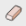
\includegraphics[width=1em]{ToolEraser}}
\end{picture}\\[-3.2em]

\normalsize
\noindent \ \,\, Eraser Tool…面の領域や線画に対して消去を行う機能です。\par
\footnotesize
\noindent [Size]: ブラシサイズを設定します。\\
\ [Type - Normal]: ブラシモードです。\\
\ [Type - Rectangular、Freehand、Polyline]: 囲んだ範囲を消去します。\\
\ [Mode - Areas]: 面の領域に対して適用します。\\
\ [Mode - Lines]: 線画に対して適用します。\\
\ [Mode - Lines \& Areas]: 面の領域と線画の両方に対して適用します。\\
\ [Selective]: チェックを入れると、既に存在する線画に対して適用できなくなります。\\
\ [Invert]: 選択した範囲以外の領域に Erase を実行します。\\
\ [Frame Range]: 複数のフレームに Erase を実行します。\\
\ [Pencil Mode]: Mode-Lines の時のみ有効です。チェックを入れると、線画を消したときにアンチエイリアスがつきません。\\[1.7em]

\normalsize
\noindent More Tools/

\large
\noindent\begin{picture}(0,0)
\put(0,0){
\includegraphics[width=1em]{ToolEdit}}
\end{picture}\\[-3.2em]

\normalsize
\noindent \ \,\, Edit Tool…カメラの選択、移動、比率の変更などの編集を行う機能です。\par
\footnotesize
\noindent ツールを使用する際には、Xsheet にてフレームやカラムを選択しておく必要があります。\\[-0.3em]

\phantomsection
\subsection*{\uline{□画像の選択した範囲をコピー/貼り付け・移動する (More Tools/)}}
\addcontentsline{toc}{subsection}{□ 画像の選択した範囲をコピー / 貼り付け・移動する (More Tools/)}

\large
\noindent\begin{picture}(0,0)
\put(0,0){
\includegraphics[width=1em]{ToolSelection}}
\end{picture}\\[-3.2em]

\normalsize
\noindent \ \,\, Selection Tool…Viewer ウィンドウ上で、画像の特定範囲を選択する機能です。\par
\footnotesize
\noindent オプションの Type を選択し、Viewer にて選択したい範囲を囲みます。複数選択が可能です。\\
矢印キーによる選択範囲内の画像の移動や、Edit メニューの Copy、Cut、Insert Paste を組み合わせることにより、複製、削除、貼り\\
付けができます。\\
異なるフレーム間でも可能です。\\
※ tlv のファイルのみ有効です。

\newpage

\phantomsection
\subsection*{\uline{□ベクター画像を編集する (More Tools/)}}
\addcontentsline{toc}{subsection}{□ ベクター画像を編集する (More Tools/)}

\noindent \\[-1.3em]

\large
\noindent\begin{picture}(0,0)
\put(0,0){
\includegraphics[width=1em]{ToolControlPointEditor}}
\end{picture}\\[-3.2em]

\normalsize
\noindent \ \,\, Control Point Editor Tool…コントロールポイントを編集して、ベクターの形を変更する機能です。\\[-0.3em]

\large
\noindent\begin{picture}(0,0)
\put(0,0){
\includegraphics[width=1em]{ToolPinch}}
\end{picture}\\[-3.2em]

\normalsize
\noindent \ \,\, Pinch Tool…ベクターのどこかをクリック&ドラッグすることで、ベクターの形を変更する機能です。\\[-0.3em]

\large
\noindent\begin{picture}(0,0)
\put(0,0){
\includegraphics[width=1em]{ToolPump}}
\end{picture}\\[-3.2em]

\normalsize
\noindent \ \ \ \ Pump Tool…ベクター線の太さを変更する機能です。変更したい範囲をクリック&ドラッグして使用しま\\
す。\\[-0.3em]

\large
\noindent\begin{picture}(0,0)
\put(0,0){
\includegraphics[width=1em]{ToolMagnet}}
\end{picture}\\[-3.2em]

\normalsize
\noindent \ \ \ \ Magnet Tool…複数のベクターを変更する機能です。変更したい範囲をクリック&ドラッグして使用しま\\
す。\\[-0.3em]

\large
\noindent\begin{picture}(0,0)
\put(0,0){
\includegraphics[width=1em]{ToolBender}}
\end{picture}\\[-3.2em]

\normalsize
\noindent \ \,\, Bender Tool…ベクター線を曲げる機能です。\\[-0.3em]

\large
\noindent\begin{picture}(0,0)
\put(0,0){
\includegraphics[width=1em]{ToolIron}}
\end{picture}\\[-3.2em]

\normalsize
\noindent \ \ \ \ Iron Tool…ベクター線のしわを修正する機能です。修正したいベクター線上でカーソルを動かして使用\\
します。\\[-0.3em]

\large
\noindent\begin{picture}(0,0)
\put(0,0){
\includegraphics[width=1em]{ToolCutter}}
\end{picture}\\[-3.2em]

\normalsize
\noindent \ \,\, Cutter Tool…ベクター線をクリックした箇所で切る機能です。\\[-0.3em]

\large
\noindent\begin{picture}(0,0)
\put(0,0){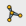
\includegraphics[width=1em]{ToolSkeleton}}
\end{picture}\\[-3.2em]

\normalsize
\noindent \ \,\, Skeleton Tool…キャラクターモデルを定義し、切り絵アニメーションとして動かす機能です。\\[-0.3em]

\large
\noindent\begin{picture}(0,0)
\put(0,0){
\includegraphics[width=1em]{ToolHook}}
\end{picture}\\[-3.2em]

\normalsize
\noindent \ \ \ \ Hook Tool…ステージスキマティックにおいて、ものを動かしたり、2 つのものをつなぐ際の基準点を定\\
義する機能です。\\[-0.3em]

\large
\noindent\begin{picture}(0,0)
\put(0,0){
\includegraphics[width=1em]{ToolTracker}}
\end{picture}\\[-3.2em]

\normalsize
\noindent \ \,\, Tracker Tool…一連の画像において、特定の部分を追跡する機能です。\\[-0.3em]

\large
\noindent\begin{picture}(0,0)
\put(0,0){
\includegraphics[width=1em]{ToolPlastic}}
\end{picture}\\[-3.2em]

\normalsize
\noindent \ \ \ \ Plastic Tool…キャラクター、もしくはその一部を変形して動かすためのメッシュを作成する機能です。\\
\\[-0.3em]

\phantomsection
\subsection*{\uline{□画像の表示に関わるツール (More Tools/)}}
\addcontentsline{toc}{subsection}{□ 画像の表示に関わるツール (More Tools/)}

\noindent \\[-2em]

\large
\noindent\begin{picture}(0,0)
\put(0,0){
\includegraphics[width=1em]{ToolZoom}}
\end{picture}\\[-3.2em]

\normalsize
\noindent \ \,\, Zoom Tool…画像を拡大・縮小する機能です。\\[-0.3em]

\large
\noindent\begin{picture}(0,0)
\put(0,0){
\includegraphics[width=1em]{ToolRotate}}
\end{picture}\\[-3.2em]

\normalsize
\noindent \ \,\, Rotate Tool…Viewer の画像表示を作業用に回転します。\\[-0.3em]

\large
\noindent\begin{picture}(0,0)
\put(0,0){
\includegraphics[width=1em]{ToolHand}}
\end{picture}\\[-3.2em]

\normalsize
\noindent \ \,\, Hand Tool…Viewer 上を移動する機能です。クリック&ドラッグして使用します。\\[-0.3em]

\phantomsection
\subsection*{\uline{□操作の取り消し (Edit/)}}
\addcontentsline{toc}{subsection}{□ 操作の取り消し (Edit/)}

\normalsize
\noindent Undo…動作のやり直しを行います。\par
\footnotesize
\noindent ※この Undo は Toonz 内のすべての作業に対して実行されます。\\[-0.3em]
\\
\normalsize
Redo…Undo で行った動作を取り消して前の状態に戻します。

\newpage

\phantomsection
\subsection*{\uline{□連番フレームの表示を送る (Edit/)}}
\addcontentsline{toc}{subsection}{□ 連番フレームの表示を送る (Edit/)}

\noindent Next Frame…Level Strip 上のフレームを 1 つ進めます。\\[-0.1em]
\\
Previous Frame…フレームを後ろに 1 つ進めます。\\[-0.1em]
\\
First Frame…フレームの先頭へ移動します。\\[-0.1em]
\\
Last Frame…フレームの最後尾へ移動します。\\[-0.1em]

\phantomsection
\subsection*{\uline{□フレームの複製・削除 (Edit/)}}
\addcontentsline{toc}{subsection}{□ フレームの複製・削除 (Edit/)}

\noindent Copy…複製する元素材を記憶します。\\[-0.1em]
\\
Cut…素材を削除・記憶します。\\[-0.1em]
\\
Insert Past…Copy/Cutで記憶させた素材を、現在選択している範囲へ貼り付け、もしくは選択しているフレー\\[-0.1em]
ムへ挿入貼り付けします。\\
\\
Paste Into…Copy したフレームを、選択したフレーム分ペーストする機能です。Level Strip のみ有効です。\\[-0.1em]
\\
Delete…選択した素材を削除します。\\[-0.1em]
\\
Insert…選択しているフレーム、もしくは Xsheet に、空のフレームを挿入します。\\[-0.1em]
\\
Select All…Selection Tool や、Level Strip で、画像もしくはフレームを全選択します。\\[-0.1em]
\\
Invert Selection…Selection Tool や、Level Strip で選択した範囲を反転させます。\\[-0.1em]
\\

\phantomsection
\subsection*{\uline{□画像の表示切り替えに関するメニュー (Checks/)}}
\addcontentsline{toc}{subsection}{□ 画像の表示切り替えに関するメニュー (Checks/)}

\noindent Transparency Check…tlv に実行すると、線のアンチエイリアスを強調し、彩色済みの領域がグレーに表示\\
されます。\par
\footnotesize
\noindent ※表示の色は Preferences で変更することができます。\\[1em]
\normalsize Black BG Check…tlvに実行すると、線画、彩色済みの領域以外の透明部分がRGB all 0の黒色に表示されます。\par
\footnotesize
\noindent ※ Transparency Check と組み合わせて使用すると、線画が白色で表示されます。\\[1em]
\normalsize Ink Check…パレットで選択したスタイルの線画を赤く表示します。\\[-0.1em]
\\
Ink\#1 Check…スタイル番号 1 の線画を赤く表示します。\\[-0.1em]
\\
Paint Check…パレットで選択したスタイルの彩色面を赤く表示します。\\[-0.1em]
\\
Fill Check…線の閉じた面積をグレーで表示します。

\newpage

\noindent Gap Check…Tape Tool でつなげる線を表示します。\\[-0.1em]
\\
Inks Only…線のみを表示します。\\[1em]

\phantomsection
\subsection*{\uline{□各種ウィンドウを表示する}}
\addcontentsline{toc}{subsection}{□ 各種ウィンドウを表示する}

\noindent Windows…各機能をフローティングウィンドウで表示するメニューです。\\[1em]

\phantomsection
\subsection*{\uline{□パレットのスタイルを編集する (Windows/)}}
\addcontentsline{toc}{subsection}{□ パレットのスタイルを編集する (Windows/)}

\noindent Style Editor…スタイルの色を編集するウィンドウです。\\[-0.5em]
\par
\footnotesize
\noindent \hskip 25.75em ①タブの切り替えにより機能が変わります。\par
\noindent \hskip 25.75em ②色の編集ウィンドウの表示・非表示の切り替えをします。\par
\noindent \hskip 25.75em ③ [Wheel]: 左で色相 (H)、右で彩度 (S) と明度 (V) をクリック&ドラッグで\par
\noindent \hskip 25.75em 変更することができます。\par
\noindent \hskip 25.75em ④ [HSV]: H(色相)S(彩度)V(明度) を編集します。\par
\noindent \hskip 25.75em ⑤ [Matte]: 透明度を編集します。\par
\noindent \hskip 25.75em ⑥ [RGB]: RGB の値を編集します。\par
\noindent \hskip 25.75em ⑦ [Color Window]: 左が現在編集中の色、右がスタイル選択時の色を表示\par
\noindent \hskip 25.75em します。\par
\noindent \hskip 25.75em ⑧ [Auto Apply]: クリックして有効にすると、色を編集したときにリアルタ\par
\noindent \hskip 25.75em イムでスタイルの色が同期します。

\large
\noindent\begin{picture}(0,0)
\put(18,-158){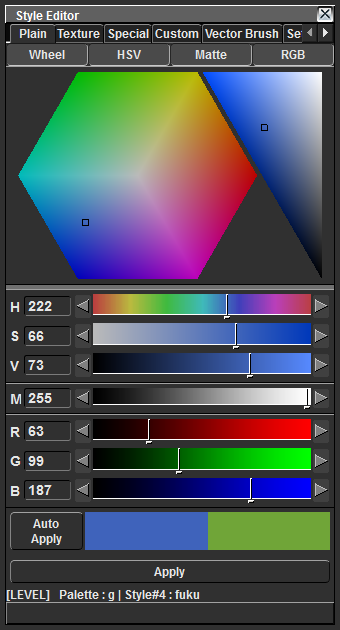
\includegraphics[width=14.5em]{PaletteStyleEditingStyleEditor}}
\color{white}
\put(13,144){●}
\put(13,132){●}
\put(35,112){●}
\put(9.5,-12){\normalsize{●}}
\put(9.5,-43){\normalsize{●}}
\put(9.5,-75){\normalsize{●}}
\put(62,-108.5){●}
\put(20,-112){●}
\color{red}
\put(13,144){①}
\put(13,132){②}
\put(35,112){③}
\put(9.5,-12){\normalsize{④}}
\put(9.5,-43){\normalsize{⑤}}
\put(9.5,-75){\normalsize{⑥}}
\put(62,-108.5){⑦}
\put(20,-112){⑧}
\end{picture}\\[12.2em]

\normalsize
\noindent Palette Gizmo…選択したスタイルに対して、色の操作を行うウィンドウです。\\[-0.5em]

\large
\noindent\begin{picture}(0,0)
\put(3,-125){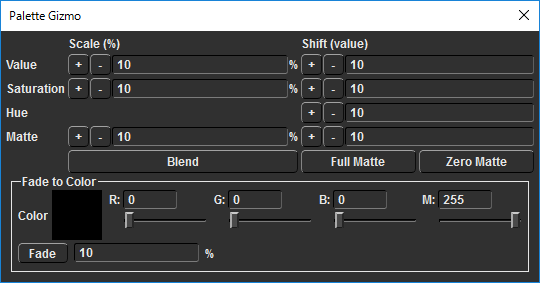
\includegraphics[width=20em]{PaletteStyleEditingPaletteGizmo}}
\color{white}
\put(-6,-31.5){\normalsize{●}}
\put(21,-23){●}
\put(125,-23){●}
\put(63,-76){●}
\put(137.5,-76){●}
\put(189,-76){●}
\put(0,-85){●}
\color{red}
\put(-6,-31.5){\normalsize{①}}
\put(21,-23){②}
\put(125,-23){③}
\put(63,-76){④}
\put(137.5,-76){⑤}
\put(189,-76){⑥}
\put(0,-85){⑦}
\end{picture}\\[-3.2em]

\footnotesize
\noindent \hskip 31.25em ① Value(明度)、Saturation(彩度)、Hue(色相)、Matte(透明度)\par
\noindent \hskip 31.25em ② [Scale(\%)]: [+][-] で現在の値から割合分、値が増減します。\par
\noindent \hskip 31.25em ③ [Shift(value)]: 現在の値から数値分、値が増減します。\par
\noindent \hskip 31.25em ④ [Blend]: スタイルを 3 つ以上選択時のみ有効です。最初のス\par
\noindent \hskip 31.25em タイルと最後のスタイルの色の中割を自動で行います。\par
\noindent \hskip 31.25em ⑤ [Full Matte]: 選択したスタイルの Matte の値を全て 255に\par
\noindent \hskip 31.25em します。\par
\noindent \hskip 31.25em ⑥ [Zero Matte]: 選択したスタイルの Matte の値を全て 0にし\par
\noindent \hskip 31.25em ます。\par
\noindent \hskip 31.25em ⑦ [Fade To Color]: Color で RGBM 値を設定し Fade Toボタン\par
\noindent \hskip 31.25em を押すと、\% の値分、色が設定した値へ近づきます。

\newpage

\normalsize
\noindent Palette…tlv に付属するパレットツールです。tpl ファイルの内容です。

\large
\noindent\begin{picture}(0,0)
\put(3,-75){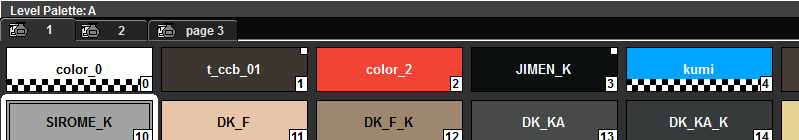
\includegraphics[width=39em]{PaletteStyleEditingLevelPalette}}
\color{white}
\put(52,6){\normalsize{●}}
\put(9,-15){●}
\put(116,-38.5){●}
\put(373.5,-38.5){●}
\put(174,-39){●}
\color{red}
\put(52,6){\normalsize{①}}
\put(9,-15){②}
\put(10,-31){\normalsize{③}}
\put(116,-38.5){④}
\put(373.5,-38.5){⑤}
\put(174,-39){⑥}
\end{picture}\\[4.9em]

\footnotesize
\noindent ①パレット名\\
②ページ: 右クリックメニューでページを追加・削除やパレットを保存できます。タブによって切り替えます。\\
③スタイル: 選択中のスタイルには白い枠が表示されます。スタイルを選択し、ctrl キー + ドラッグすると移動ができます。\\
④スタイル名: ダブルクリックして名前を変更することができます。\\
⑤ Matte の値に順じて、下部がチェッカー表示になります。値が小さいほどチェッカーが濃く表示されます。\\
⑥スタイル番号: スタイルの並びを変更しても番号は変化しません。

\large
\noindent\begin{picture}(0,0)
\put(3,-115){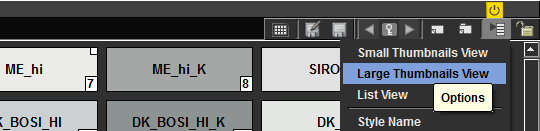
\includegraphics[width=39em]{PaletteStyleEditingViewOptions}}
\color{white}
\put(241,-20){●}
\put(269,-20){●}
\put(292,-20){●}
\put(335,-20){●}
\put(377,-20){●}
\put(402,-20){●}
\put(423.5,-30.5){●}
\put(455.5,-20){●}
\color{red}
\put(241,-20){①}
\put(269,-20){②}
\put(292,-20){③}
\put(335,-20){④}
\put(377,-20){⑤}
\put(402,-20){⑥}
\put(423.5,-30.5){⑦}
\put(455.5,-20){⑧}
\end{picture}\\[8.3em]

\footnotesize
\noindent ① [Palette]: Studio Palette へドラッグ&ドロップすることにより、Current Palette を Studio Palette へ新規ページとして追加します。\\
② [Save Palette As]: Current Palette を別名保存します。\\
③ [Save Palette]: Current Palette を上書き保存します。\\
④ [Set Key]: key color chip を設定することにより、1 つの tpl 内に複数の色を作成することができます。\\
⑤ [New Style]: スタイルを1つ追加します。\\
⑥ [New Page]: パレットのページを追加します。\\
⑦パレットの表示の切り替えメニューです。\\
⑧ [Lock Palette]: パレット内容の編集を可能 / 不可能かを切り替えることができます。\\

\phantomsection
\subsection*{\uline{□ Studio Palette について}}
\addcontentsline{toc}{subsection}{□ Studio Palette について}

\normalsize
\noindent Studio Palette…色見本となるパレットを表示するウィンドウです。\\

\phantomsection
\subsection*{\uline{□ Studio Palette 内でフォルダを作成・削除、新規パレットを作成する。}}
\addcontentsline{toc}{subsection}{□ Studio Palette 内でフォルダを作成・削除、新規パレットを作成する。}

\vspace{1.5em}

\noindent \hskip 17em Toonz Palettes…\$TOONZSTUDIOPALETTES で指定されたフォルダ (通常は\par
\noindent \hskip 17em Stuff フォルダ内の studiopalettes フォルダ) の内容が表示されます。\par
\noindent \hskip 17em Project Palettes…+palettes プロジェクトフォルダの内容が表示されます。\\
\par
\footnotesize
\noindent \hskip 21.25em ※ Toonz Palette はスタジオ全体で使用するパレット、Project Palette は各作品で使用\par
\noindent \hskip 21.25em するパレットです。

\large
\noindent\begin{picture}(0,0)
\put(7,-69){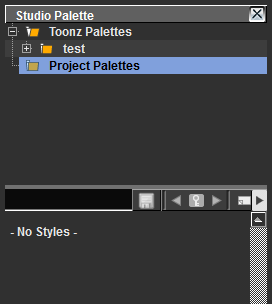
\includegraphics[width=12.9em]{StudioPaletteProjectPalettes}}
\linethickness{0.1em}
\color{red}
\put(162,100){\line(-5,-1){75}}
\put(162,67){\line(-1,0){75}}
\end{picture}

\newpage

\large
\noindent\begin{picture}(0,0)
\put(15,-177){\includegraphics[width=12.4em]{StudioPaletteNewPalette}}
\linethickness{0.1em}
\color{red}
\put(167,-35){\line(-6,1){66}}
\end{picture}\\[0.3em]

\footnotesize
\noindent \hskip 22em New Palette…パレットを新規作成します。\par
\noindent \hskip 22em New Folder…フォルダを新規作成します。\par
\noindent \hskip 22em Delete Folder…フォルダを削除します。フォルダの中にあるパレットも削除します。\par
\noindent \hskip 22em Search for Palette…パレットを検索することができます。\\[10.5em]

\noindent \,Studio Palette に保存されたスタイルからコピーしたスタイルは、コピー元のスタイルとリンクします。\\
・リンクのあるスタイルは右上に四角いマークが表示されます。リンクしたスタイルの色を Studio Palette に登録された色から変更す\\
ると、斜線が表示されます。\\
・スタイルを選択し、[ 右クリックメニュー /Get Color from Studio Palette] を選択すると、リンク元の Studio Palette に登録されたス\\
タイルの色に戻ります。\par
\noindent \hskip 27em ・リンクを外したい場合は、[ 右クリックメニュー /Remove Links] を選択\par
\noindent \hskip 27em すると Studio Palette とのリンクが切れます。

\large
\noindent\begin{picture}(0,0)
\put(3,-44){\includegraphics[width=17.4em]{StudioPaletteRemoveLinks}}
\end{picture}

\newpage

\phantomsection
\subsection*{\uline{□画像を表示する (Windows/)}}
\addcontentsline{toc}{subsection}{□ 画像を表示する (Windows/)}

\normalsize
\noindent Combo Viewer…画像を表示するウィンドウです。\par
\footnotesize
\noindent ウィンドウ内の右クリックメニューで、表示の変更などが行えます。\\
\par
\noindent \uline{【ビューモードのメニュー】}\\
① [Camera Stand View]: 画像の元サイズで表示します。通常はこちらを選択して作業します。\\
② [3D View]: カメラと画像素材の位置関係を 3D で表示します。\\
③ [Freeze]: Preview モード表示中、画像やエフェクトに変化があっても Preview 表示を更新しません。\\
④ [Preview]: 画像を Output Settings で設定したカメラサイズ、エフェクトも適用した状態で表示します。

\large
\noindent\begin{picture}(0,0)
\put(279,-34){\includegraphics[width=13.7em]{ViewingTheImageViewModeMenu}}
\put(104,-232){\includegraphics[width=22.4em]{ViewingTheImageViewer}}
\put(3,-280){\includegraphics[width=39em]{ViewingTheImageConsoleMenu}}
\linethickness{0.1em}
\color{red}
\put(343.5,7){\normalsize{①}}
\put(353.5,7){\normalsize{②}}
\put(376.5,7){\normalsize{③}}
\put(390,7){\normalsize{④}}
\put(3,-251){\normalsize{①}}
\put(20,-251){\normalsize{②}}
\put(38,-251){\normalsize{③}}
\put(55,-251){\normalsize{④}}
\put(94,-251){\normalsize{⑤}}
\put(111.5,-251){\normalsize{⑥}}
\put(128.5,-251){\normalsize{⑦}}
\put(149,-251){\normalsize{⑧}}
\put(166,-251){\normalsize{⑨}}
\put(182.5,-251){\normalsize{⑩}}
\put(199,-251){\normalsize{⑪}}
\put(218,-251){\normalsize{⑫}}
\put(235,-251){\normalsize{⑬}}
\put(253,-251){\normalsize{⑭}}
\put(287,-251){\normalsize{⑮}}
\put(325,-251){\normalsize{⑯}}
\put(355,-251){\normalsize{⑰}}
\put(421.5,-251){\normalsize{⑱}}
\put(272,05){\line(1,0){166}}
\put(272.5,05){\line(0,-1){39}}
\put(437.5,05){\line(0,-1){39}}
\put(272,-34){\line(1,0){166}}
\put(341,-34){\line(-1,-4){3.7}}
\put(180,-254){\line(-1,6){4.6}}
\put(-3.5,-254){\line(1,0){469.5}}
\put(-3,-254){\line(0,-1){26}}
\put(465.4,-254){\line(0,-1){26}}
\put(-3.5,-280){\line(1,0){469.5}}
\end{picture}\\[22.8em]

\footnotesize
\noindent \uline{【コンソールのメニュー】}\\
①オプションの表示 / 非表示を切り替え\\
②表示している画像を Output Settings で設定したフォーマットで保存します。Preview モードのみ有効です。\\
③表示している画像の 1 フレームをメモリに記憶します。この機能は④で使用します。\\
④「③」で記憶したフレームと、再度プレビューしたフレームとを比較表示します。\\
⑤背景色を RGB all 255 で表示\\
⑥背景色を RGB all 0 で表示\\
⑦背景色を Matte 0 で表示\\
⑧先頭のフレームへ移動\\
⑨フレームを 1 つ戻る\\
⑩フレームを一時停止\\
⑪フレームを再生\\
⑫フレームをループ再生\\
⑬フレームを 1 つ進む\\
⑭最後のフレームへ移動\\
⑮ R,G,B,Matte ボタンがあり、クリックするとそれぞれの色情報のみ表示\\
⑯画像のヒストグラムを表示\\
⑰キーフレームを設定します。左右のボタンでキーフレームに移動します。\\
⑱再生時のフレームレートを指定します。

\newpage

\phantomsection
\subsection*{\uline{□タイムシートの編集を行う (Windows/)}}
\addcontentsline{toc}{subsection}{□ タイムシートの編集を行う (Windows/)}

\normalsize
\noindent Xsheet…tlv や tif などの画像ファイルを配置して、各作業を行うウィンドウです。\par
\footnotesize
\noindent 左右がセルの重ね順、上下が時間軸を表示しています。\\
\par
\noindent \hskip 22.5em ①プレビュー時の表示 / 非表示\par
\noindent \hskip 22.5em ② Camera Stand の表示 / 非表示\par
\noindent \hskip 22.5em ③カラムの先頭フレームをサムネール表示\par
\noindent \hskip 22.5em ④ペグバーの種類を表示\par
\noindent \hskip 22.5em ⑤ Column・Cells を表示

\large
\noindent\begin{picture}(0,0)
\put(7,-82){\includegraphics[width=13.4em]{TimeSheetEditingXsheet}}
\color{white}
\put(64,63.5){●}
\put(64,51.5){●}
\put(64,33.5){●}
\put(64,16.4){●}
\put(64,-23){●}
\color{red}
\put(64,63.5){①}
\put(64,51.5){②}
\put(64,33.5){③}
\put(64,16.4){④}
\put(64,-23){⑤}
\end{picture}\\[6em]

\footnotesize
\noindent \uline{【右クリックメニュー】}\\
※以下の項目は選択した Cells に対して適用されます。\\
\ [Step]: コマ打ちを変更することができます。例) Step2 = 2 コマ打ち\\
\ [Each]: 数値分間引いてカットします。例) Each2 1,2,3,4,5 → 1,3,5\\
\ [Reverse]: 逆の順序にします。\\
\ [Swing]: Reverse したものを追加します。\\
\ [Random]: ランダムに並べ替えます。\\
\ [Repeat]: 選択分追加コピーします。\\
\ [Roll Up]: 1 フレーム繰り上げます。\\
\ [Roll Down]: 1 フレーム繰り下げます。\\
\ [Time Stretch]: 数値分圧縮間引きします。\\
\\
\ [Replace Level]: 現在の Cells と新規に Load した素材を入れ替えます。\\
\ [Revert to Cleaned Up]: 選択したCellsをNo paintのデータで置き換えます。\\
\ [Info]: 選択した画像の情報を表示します。\\
\ [View]: 選択した画像を表示します。

\large
\noindent\begin{picture}(0,0)
\put(283,-5){\includegraphics[width=16.6em]{TimeSheetEditingRightClickMenu}}
\end{picture}\\[-1.2em]

\phantomsection
\subsection*{\uline{□ペイントの際に使用する色見本を表示する (Windows/)}}
\addcontentsline{toc}{subsection}{□ ペイントの際に使用する色見本を表示する (Windows/)}

\normalsize
\noindent Color Model…ペイントの際に色見本となる tlv を Load します。画像から色を抽出することができるウィン\\
ドウです。\\[-0.5em]
\par
\footnotesize
\noindent \uline{【右クリックメニュー】}\\
\ [Load Color Model]: tlvを選択するブラウザが表示されます。ファイルを選択してColor Modelウィンドウに読み込みます。※複数フレー\\
ムの tlv を Load した場合、Console でフレームの移動ができます。Warning ウィンドウが表示されるので、どちらかのメニューを選択\\
します。\\
・Overwrite the destination palette…選択したcolor modelのtplを、現在選択しているtlvへ上書きします。color model (見本となる\\
tlv) は、color model の色で Load されます。\\
・Keep the destination palette and apply it to the color model…選択したcolor modelのtpl は Loadされません。現在作業中のtplがそ\\
のまま使用されます。color model は、現在作業中の色で Load されます。\\
\\
\ [Use Current Frame]: 現在選択中の tlv フレームを Color Model として Load します。\\
\ [Remove Color Model]: Color Model を消去します。\\
※ tga 形式のファイルを読み込んで、画像から RGB 値を抽出することも可能です。

\newpage

\phantomsection
\subsection*{\uline{□ファイルをブラウズする (Windows/)}}
\addcontentsline{toc}{subsection}{□ ファイルをブラウズする (Windows/)}

\normalsize
\noindent File Browser…ファイルをブラウズするウィンドウです。\par
\footnotesize
\noindent ウィンドウの詳細は「ファイルブラウザのインターフェイス」 (p.4) を参照してください。\\
このウィンドウではファイルの Load ができません。ディレクトリの作成、ファイル情報の表示などは可能です。\\

\phantomsection
\subsection*{\uline{□ファイルをブラウズする (Windows/)}}
\addcontentsline{toc}{subsection}{□ ファイルをブラウズする (Windows/)}

\normalsize
\noindent Level Strip…tlv のフレームを表示、編集するウィンドウです。\\
\par
\footnotesize
\noindent \hskip 21.25em ① Scene に Load している tlv を選択できます。「*」 が表示されているファイルは、変\par
\noindent \hskip 21.25em 更が加えられて保存をしていない状態です。\par
\noindent \hskip 21.25em ②フレーム番号\par
\noindent \hskip 21.25em ③現在選択中のフレームは赤い枠が表示されます。内側に表示される赤い枠は、\par
\noindent \hskip 21.25em Viewer 上での表示範囲です。枠をドラッグすると View の位置を変更することができ\par
\noindent \hskip 21.25em ます。画像に編集を加えると、リアルタイムで表示が更新されます。\\
\par
\noindent \hskip 20.75em 【右クリックメニュー】\par
\noindent \hskip 21.25em [Select All]: 全てのフレームを選択します。\par
\noindent \hskip 21.25em [Invert Selection]: 選択したフレームがすべて反転選択されます。\par
\noindent \hskip 21.25em [Cut]: 選択したフレームをカットします。\par
\noindent \hskip 21.25em [Copy]: 選択したフレームをコピーします。\par
\noindent \hskip 21.25em [Insert Paste]: Copy で記憶した素材を選択しているフレームへ挿入ペーストします。\par
\noindent \hskip 21.25em [Paste Into]: Copy したフレームを、選択したフレーム分ペーストします。\par
\noindent \hskip 21.25em [Merge]: Copy したフレームを、現在選択している tlv のフレーム番号に対応した場所\par
\noindent \hskip 21.25em へペーストします。\par
\noindent \hskip 21.25em [Insert]: 選択しているフレーム数分、空 (から) のフレームを挿入します。\par
\noindent \hskip 21.25em [Delete]: 選択したフレームの画像を消去します。フレームは消去されません。\par
\noindent \hskip 21.25em [Duplicate Drawing]: 選択したフレーム数分、フレームの下にコピー&ペーストします。\par
\noindent \hskip 21.25em [Reverse]: 選択したフレームの画像内容が逆の順序になります。例) 1,2,3 → 3,2,1\par
\noindent \hskip 21.25em [Swing]: 選択したフレームを Reverse 追加します。例) 1,2,3,4 → 1,2,3,4,3,2,1\par
\noindent \hskip 21.25em [Step2~4]: 選択したフレームを数値分増やします。例) Step2 1,2,3 → 1,1,2,2,3,3\par
\noindent \hskip 21.25em [Each2~4]: 選択したフレームを数値分間引きカットします。例) Each2 1,2,3,4 →1,3\par
\noindent \hskip 21.25em [Expose in Xsheet]: 選択したフレームを Xsheet に追加します。\par
\noindent \hskip 21.25em [Add Frames]: 専用のウィンドウが表示され、数値入力すると空 (から) のフレームを\par
\noindent \hskip 21.25em 追加します。\par
\noindent \hskip 21.25em [Renumber]: 選択したフレームのフレーム番号を変更します。\par
\noindent \hskip 21.25em [Revert to Cleaned Up]: 選択したフレームを No paint のデータで上書きします。\par
\noindent \hskip 21.25em Cleanup 直後の画像に戻ります。

\large
\noindent\begin{picture}(0,0)
\put(3,30){\includegraphics[width=13.4em]{TLVFrameViewingLevelStrip}}
\color{white}
\put(41,367){●}
\put(94,279){●}
\color{red}
\put(41,367){①}
\put(94,279){②}
\put(52,306){\normalsize{③}}
\end{picture}\\[0.5em]

\normalsize
\noindent Toolbar…Tool を表示するウィンドウです。\par
\footnotesize
\noindent 各機能については「Tools」 (p.13~) を参照してください。\\[-0.5em]
\par
\normalsize
\noindent Tool Option Bar…Tool Option Bar を表示するウィンドウです。\par
\footnotesize
\noindent 機能については各 Tool の説明を参照してください。\\[-0.5em]
\par
\normalsize
\noindent Reset to Default Rooms…ルームの設定を初期状態にリセットする機能です。\\[-0.5em]
\\
Batch Servers…Batch の計算をどのマシンで行うかを設定するウィンドウです。

\newpage

\phantomsection
\subsection*{\uline{□連番画像を動画でプレビューする (Windows/)}}
\addcontentsline{toc}{subsection}{□ 連番画像を動画でプレビューする (Windows/)}

\normalsize
\noindent Flipbook…動画を再生、保存するウィンドウです。\par
\footnotesize
\noindent tif、tlv、rgb などの画像ファイルを Load し、アニメーションさせることができます。\\
\par
\normalsize
\noindent Viewer のコンソールメニューでも、表示している連番画像を動画で再生可能です。\\
\\
Function Editor…Xsheet 上のカメラやカラムを、数値入力により設定するウィンドウです。\\[1em]
Scene Cast…現在 Scene に Load されている画像ファイルを表示するウィンドウです。\par
\footnotesize
\noindent Xsheet 上では非表示でも、Scene Cast に表示されているファイルは Scene の中に Load されています。\\
※ Xsheet 上からセルを削除しても Scene Cast に登録されているファイルは Load されたままの状態です。\\
ファイルの登録を取り消すには、Cast ファイルを選択し、右クリックメニュー /[Remove Level] を実行します。\\
\par
\normalsize
\noindent Schematic…Xsheet 上での素材、カメラ、エフェクトの状態をフローチャートで表示するウィンドウです。\\
\\
Tasks…Batches のタスクを表示するウィンドウです。\par
\footnotesize
\noindent tnz を Load してバッチ処理を行うことができます。\\
\\

\phantomsection
\subsection*{\uline{□環境設定・キーボードショートカットを変更する (Customize/)}}
\addcontentsline{toc}{subsection}{□ 環境設定・キーボードショートカットを変更する (Customize/)}

\normalsize
\noindent Preferences…Toonz 全体の環境設定を行うメニューです。\\
\\
Configure Shortcuts…Toonz のキーボードショートカットを設定するメニューです。\\
\\
Scene Settings…フレームレートや、カメラの背景色などの設定を行うメニューです。\\

\phantomsection
\subsection*{\uline{□各種表示メニュー (Customize/)}}
\addcontentsline{toc}{subsection}{□ 各種表示メニュー (Customize/)}

\normalsize
\noindent View…Combo Viewer で表示する各種メニューです。\par
\footnotesize
\noindent [Camera Box]: Output Settingsで設定したカメラサイズを、Viewer上に赤色の破線で表示します。*InknPaint Roomでtlvを選択して\\
いるときには表示されません。\\
\ [Table]: 背景の Camera Stand の表示です。\\
\ [Field Guide]: マス目状のガイド表示です。単位は Inch です。\\
\ [Safe Area]: Camera Box 表示時に、実際にスクリーンやテレビで表示される領域の表示です。\\
\ [Camera BG Color]: 画像ファイルの下に背景を表示します。大きさは Output Settings で設定したカメラサイズです。\\

\phantomsection
\subsection*{\uline{□ウィンドウレイアウトを固定する (Customize/)}}
\addcontentsline{toc}{subsection}{□ ウィンドウレイアウトを固定する (Customize/)}

\normalsize
\noindent Lock Room Panes…ウィンドウレイアウトの固定 / 解除の切り替えメニューです。

\newpage

\phantomsection
\subsection*{\uline{□ tlv ファイルを tlv 以外のファイル形式に変換する}}
\addcontentsline{toc}{subsection}{□ tlv ファイルを tlv 以外のファイル形式に変換する}

\footnotesize
\noindent OpenToonz で仕上げ作業済みのファイルを、他のソフトを使用して撮影する・ファイルを開くなどの場合、ファイルのコンバート (変\\
換) を行います。\\[-0.5em]
\par
\normalsize
\noindent 1. ファイルブラウザ上でコンバートしたいファイルを右クリックし [Convert] を選択します。

\large
\noindent\begin{picture}(0,0)
\put(117,-153){\includegraphics[width=19.2em]{TLVFileConversionToOtherFileFormats}}
\color{white}
\put(132.5,-92){\small{●}}
\put(132.5,-101){\small{●}}
\color{red}
\put(108,-44){\footnotesize{①}}
\put(108,-52.5){\footnotesize{②}}
\put(108,-61){\footnotesize{③}}
\put(108,-69.5){\footnotesize{④}}
\put(108,-82){\footnotesize{⑤}}
\put(132.5,-92){\small{⑥}}
\put(132.5,-101){\small{⑦}}
\end{picture}\\[11.75em]

\footnotesize
\noindent ①作成するフレーム範囲を入力します。\\
②作成するファイルの保存先を選択します。\\
③ファイル名を入力します。\\
④ファイル形式を選択します。\\
⑤背景色を設定します。通常は RGB all 255 (白) です。\\
⑥チェックを入れると、保存先に既に同じファイルが存在している場合に、そのファイルには上書きせず新たにファイルを作成します。\\
⑦チェックを入れると、変換前の tlv のファイル名のフレーム番号の前に付いている [.(ドット)] を削除することができます。\\
例) File Name を "A"  \ Remove dot before frame number を "オフ" の場合: A.0001.tga, A.0002.tga, A.0003.tga....\\
例) File Name を "A\_"  Remove dot before frame number を "オン" の場合: A\_0001.tga, A\_0002.tga, A\_0003.tga....\\
※ 変換後のファイル形式に tlv を選択していない場合のみ、機能が有効になります。\\
※ OpenToonz は、レベル名と 4 ケタのフレーム番号の間に "." (ドット) 又は "\_"  (アンダースコア)がある形式のファイルを、1連の\\
レベルとして認識します。\\
\par
\normalsize
\noindent 2.[Convert] をクリックすると、Convert を開始します。

\newpage

\phantomsection
\section*{\uline{■ PltEdit}}
\addcontentsline{toc}{section}{■ PltEdit}

\footnotesize
\noindent PltEdit ルームでは、背景素材とセルを重ねたファイルを作成し、パレットの編集を行います。仕上げ工程の中でも、主に色を決める場\\
面で使用します。\\

\phantomsection
\subsection*{\uline{□色指定を行うためのシートファイルの作成}}
\addcontentsline{toc}{subsection}{□ 色指定を行うためのシートファイルの作成}

\footnotesize
\noindent 色を決める際に、必要なシートのファイルを作成します。\\
\par
\normalsize
\noindent 1. BG (背景素材) のファイルとペイントされた tlv ファイルをシート上に読み込みます。\par
\footnotesize
\noindent Xsheet 上の並べたい場所のカラムを選択し、Load Level で tlv ファイルを読み込みます。\\
Xsheet のカラム 1 (最背面となる素材) には BG を読み込みます。その他の Book 素材や各セルは実際のタイムシート通りの重ね順でファ\\
イルを読み込みます。位置合わせのためにレイアウトのファイルも読み込みます。\\
\par
\normalsize
\noindent 2.BG の位置をレイアウトファイルの位置に合わせて移動します。\par
\footnotesize
\noindent BG がレイアウトとずれている場合は、位置合わせを行います。\\
レイアウトと BG のみを表示にします。\\
動かしたい方のファイル (BG) を選択し、Edit ツールを使用してレイアウトに合わせて動かします。\\
※レイアウトファイルなど、プレビュー時に表示する必要のないセルは、Xsheet上の各セルの上部にある[Preview\,\,Visibility Toggle]\\
をクリックして表示 / 非表示を切り替えることができます。\\
\par
\normalsize
\noindent 3.Book がある場合は、BG と同様に位置を動かします。\par
\footnotesize
\noindent [Windows/Other Windows/Schematic] を選択し、Schematic ウィンドウを表示します。\\
カラム 1 (BG) の数値で他の Book の位置合わせをするには、Stage Schematic 上で、Book の青い●をクリック \& ドラッグしてカラム\\
1 の赤い●につなげます。\\
※プレビュー時に Book に白いエッジが表示される場合は FX Schematic 上で Book を選択し、[右クリックメニュー /Insert FX/Layer\\
Blending/Premultiply] を選択します。Book を選択し Level Settings の [Premultiply] にチェックを入れることでもプレビュー時のエッ\\
ジを消すことができます。\\
\par
\normalsize
\noindent 4.Style Editor や Studio Palette などを使用してスタイルを編集します。\par
\footnotesize
\noindent RGB Picker ツールで背景画像から色を抽出することもできます。\\
プレビューを実行し、処理をかけた状態の画面を確認することも可能です。\\
\\

\phantomsection
\subsection*{\uline{□必要なフレームのみを表示する}}
\addcontentsline{toc}{subsection}{□ 必要なフレームのみを表示する}

\normalsize
\noindent 必要な番号のみを Xsheet に並べるか、Sub-Xsheet を使用し、必要なシート番号のみをプレビューすること\\
も可能です。\\
\par
\noindent \hskip -0.5em 【Sub-Xsheet の作成方法】\\
含みたいセルを全て選択し、[右クリックメニュー /Collapse] を選択します。以下のアラートウィンドウが\\
表示されます。\par
\footnotesize
\noindent ・Include relevant pegbars in the sub-xsheet as well. …Pegbar の情報も Sub-Xsheet に含む。\\
・Include only selected columns in the sub-xsheet. …Pegbar の情報は Sub-Xsheet に含まない。\\
Sub-Xsheet は Xsheet 上に紫色で表示されます。\\
Sub-Xsheet に畳んだ状態で、プレビューするシート番号を打ち込みます。

\newpage

\phantomsection
\subsection*{\uline{□ダブラシ影などを透けた表示でプレビューする}}
\addcontentsline{toc}{subsection}{□ ダブラシ影などを透けた表示でプレビューする}

\footnotesize
\noindent 簡易的に Schematic 上でエフェクトを追加します。\\[-0.5em]
\par
\small
\noindent 1.処理をかけたいセルをコピーして Xsheet に同じセルを二つ並べます。\\
\\
2.Fx Schematic 上で、セルを選択し、それぞれ[右クリックメニュー/Insert FX/Toonz Level/Palette Filter]を選択します。\\
FX が追加されたら、FX をダブルクリックします。設定画面が表示されます。\\
\par
\footnotesize
\noindent \hskip 30.25em [Color Indexes]: ダブラシ影のスタイル番号を入力します。\par
\noindent \hskip 30.25em [Action]: 一方は keep を選択し、もう一方のセルは Deleteを選択\par
\noindent \hskip 30.25em します。

\large
\noindent\begin{picture}(0,0)
\put(3,-120){\includegraphics[width=19.3em]{PreviewingTransparentDisplayFxSchematic}}
\end{picture}\\[9.25em]

\small
\noindent 3.Action の項目で Keep を選択した方のセルの FX を選択し、[右\\
クリックメニュー /Insert FX/Layer\_Blending/Transparency]を選\\
択します。ダブルクリックで処理の強さの設定を変更することも\\
できます。\par
\footnotesize
\noindent プレビューした際に、ダブラシ処理のかかった表示になります。\\
他のセルの影と重なってしまい二重に表示されてしまう場合は、コピーし\\
たダブラシ影用のセルをSub-Xsheetにまとめ、そのSub-Xsheetに対して\\
Transparency処理をかけると、影が二重に表示されることなく透けた処理\\
をかけることができます。

\large
\noindent\begin{picture}(0,0)
\put(271,-4){\includegraphics[width=16.8em]{PreviewingTransparentDisplayTransparency}}
\end{picture}

\end{document}